%% 
%% ACS project dissertation template. 
%% 
%% Currently designed for printing two-sided, but if you prefer to 
%% print single-sided just remove ",twoside,openright" from the 
%% \documentclass[] line below. 
%%
%%
%%   SMH, May 2010. 


\documentclass[a4paper,12pt,twoside,openright]{report}


%%
%% EDIT THE BELOW TO CUSTOMIZE
%%

\def\authorname{Zubair Nabi\xspace}
\def\authorcollege{Robinson College\xspace}
\def\authoremail{Zubair.Nabi@cl.cam.ac.uk}
\def\dissertationtitle{Mission Control: Enabling Efficient and Heterogeneous Data Transfers
in Data Intensive Computing}
\def\wordcount{13956}


\usepackage{epsfig,graphicx,parskip,setspace,tabularx,xspace,epstopdf,url,caption,subcaption,float,listings,color} 
\graphicspath{{./Figures/}}
\definecolor{javared}{rgb}{0.6,0,0} % for strings
\definecolor{javagreen}{rgb}{0.25,0.5,0.35} % comments
\definecolor{javapurple}{rgb}{0.5,0,0.35} % keywords
\definecolor{javadocblue}{rgb}{0.25,0.35,0.75} % javadoc

%% START OF DOCUMENT
\begin{document}


%% FRONTMATTER (TITLE PAGE, DECLARATION, ABSTRACT, ETC) 
\pagestyle{empty}
\singlespacing
% title page information
\begin{titlepage} 

\begin{center}
\noindent
\huge
\dissertationtitle \\
\vspace*{\stretch{1}}
\end{center}

\begin{center}
\noindent
\huge
\authorname \\
\Large
\authorcollege      \\[24pt]

\includegraphics{CUni3.eps}
\end{center}

\vspace{24pt} 

\begin{center}
\noindent
\large
{\it A dissertation submitted to the University of Cambridge \\ 
in partial fulfilment of the requirements for the degree of \\ 
Master of Philosophy in Advanced Computer Science\\
(Option B)} 
\vspace*{\stretch{1}}
\end{center}

\begin{center}
\noindent
University of Cambridge \\
Computer Laboratory     \\
William Gates Building  \\
15 JJ Thomson Avenue    \\
Cambridge CB3 0FD       \\
{\sc United Kingdom}    \\
\end{center}

\begin{center}
\noindent
Email: \authoremail \\
\end{center}

\begin{center}
\noindent
\today
\end{center}

\end{titlepage} 

\newpage
\vspace*{\fill}

\onehalfspacing
\newpage
{\Huge \bf Declaration}

\vspace{24pt} 

I \authorname of \authorcollege, being a candidate for the M.Phil in
Advanced Computer Science, hereby declare that this report and the
work described in it are my own work, unaided except as may be
specified below, and that the report does not contain material that
has already been used to any substantial extent for a comparable
purpose.

\vspace{24pt}
Total word count: \wordcount

\vspace{60pt}
\textbf{Signed}: 

\vspace{12pt}
\textbf{Date}:


\vfill

This dissertation is copyright \copyright 2010 \authorname. 
\\
All trademarks used in this dissertation are hereby acknowledged.



\newpage
\vspace*{\fill}

\onehalfspacing
\newpage
{\Huge \bf Acknowledgements}

\vspace{24pt} 

Dr Steven Hand, Dr Anil Madhavapeddy

Dr Kenneth Birman, Malte Schwarzkopf, Derek Murray

Family, friends, Natalie

\vfill

\newpage
\vspace*{\fill}

\singlespacing
\newpage
{\Huge \bf Abstract}
\vspace{24pt} 


This is the abstract. Write a summary of the whole thing. Make 
sure it fits in one page. 


\newpage
\vspace*{\fill}


\pagenumbering{roman}
\setcounter{page}{0}
\pagestyle{plain}
\tableofcontents
\listoffigures
\listoftables

\onehalfspacing

%% START OF MAIN TEXT 

\chapter{Introduction}
\pagenumbering{arabic} 
\setcounter{page}{1} 

Over the course of the last decade, proliferation in web applications (Facebook,
Twitter etc.), and scientific computing (sensor networks, high energy physics,
etc.) has resulted in an unparalleled surge in data on the exabyte scale.
Consequently, the need to store and analyze this data has engendered an
ecosystem of distributed file systems~\cite{Ghemawat:2003:GFS}, structured and
unstructured data stores~\cite{Chang:2006:BDS,DeCandia:2007:DAH}, and
data-intensive computing
frameworks~\cite{Dean:2004:MSD,Isard:2007:DDD,Murray:2011:CUE}. These
``shared-nothing'' frameworks are mostly run in massive data centers with tens
of thousands of servers and network elements. These data centers are globally
distributed, for diversity and redundancy, and run a wide-variety of loads;
including user-facing applications, such as email; custom enterprise
applications, such as authentication services; and large-scale batch-processing
applications, such as web indexing~\cite{Benson:2010:NTC}. The goal of each data
center is to provide a multi-tenant\footnote{Multi-tenancy applies to both
public clouds, such as Amazon EC2 and Microsoft Azure, where the resources are
shared by paying customers and to private clouds, maintained by Google,
Facebook, etc., where different departments share the same infrastructure.}
environment for energy-, power-, space-, and cost-efficient computation, and
storage at scale~\cite{Katz:2009:TTB}.

Typically, data centers are built using commodity, off-the-shelf servers and
switches to find a sweet spot between performance and cost, and to leverage
economies of scale~\cite{Barroso:2003:WSP}. Servers in this model store or
process a \emph{chunk} of data, with redundancy ensured via replication without
any cluster/data center wide memory or storage area network (SAN). Due to their
commodity nature, servers and network elements are failure-prone and a failure
in say, a \emph{core switch} can bring down the entire network. Therefore,
storage and processing frameworks use a range of methods to deal with this,
including replication, re-execution, and speculative execution. On the network
side, end-hosts running TCP/IP are connected through cheap switches and wired
links, although wireless~\cite{Halperin:2011:ADC} and
optical~\cite{Wang:2010:CPO,Farrington:2010:HHE} links have recently been
explored. Most data centers are provisioned with 1Gbps and 10Gbps switches with
L2 Ethernet switched fabric interconnects as opposed to fabrics from the high
performance computing community such as InfiniBand. Likewise, due to the
prohibitive cost of high-end switches and routers, as opposed to commodity
off-the-shelf hardware, bandwidth is a constrained resource in the data center.
To ensure optimum utilization, subject to organizational goals, oversubscription
factors\footnote{Oversubscription factor is defined as ``the ratio of worst-case
achievable aggregate bandwidth among the end hosts to the total bisection
bandwidth of a particular communication topology"~\cite{Al-Fares:2008:SCD}.} in
real data centers vary significantly:
Some are as low as 2:1 while some can get as high as
147:1~\cite{Benson:2010:NTC}. In the cluster hierarchy, bandwidth increases from
the edge of the network towards the core (off-rack oversubscription). As a
result of off-rack oversubscription, applications are designed to keep
cross-rack communication to a minimum~\cite{Dean:2004:MSD}.

Concurrently, the emergence of cloud computing has resulted in multi-tenant data
centers in which user applications have wide-varying requirements and
communication patterns. Applications range from low-latency query jobs to
bandwidth-hungry batch processing jobs~\cite{Alizadeh:2010:DCT}. In addition,
applications exhibit one-to-many, many-to-one, and many-to-many communication
patterns. In order to ensure better fault-tolerance, scalability, and end-to-end
bandwidth in data center networks, several new
topologies~\cite{Al-Fares:2008:SCD,Guo:2008:DSF,Guo:2009:BHP,Greenberg:2009:VSF}
have been proposed to replace the status quo: a hierarchical 2/3-level tree
which connects end-hosts through \emph{top-of-rack} (or \emph{aggregation}), and
\emph{core} switches. In the same vein,
L2~\cite{Mudigonda:2010:SCD,Vattikonda:2012:PTD} and
L3/L4~\cite{Alizadeh:2010:DCT,Vasudevan:2009:SEF,Raiciu:2010:DCN,Wilson:2011:BNL,Wu:2010:IIC}
protocols, topologies and design
frameworks~\cite{Singla:2011:JND,Al-Fares:2008:SCD,Guo:2008:DSF,Guo:2009:BHP,Greenberg:2009:VSF,Mudigonda:2011:TFC,Chen:2010:GAA},
and control and virtualization
planes~\cite{NiranjanMysore:2009:PSF,Mudigonda:2011:NSM,Guo:2010:SDC,Ballani:2011:TPD,Shieh:2011:SDC,Rodrigues:2011:GSB,Al-Fares:2010:HDF}
for data center communication and resource allocation have also experienced
innovation, focusing on some combination of high bandwidth, fairness,
fault-tolerance, and scalability.

In this thesis, we explore a new point in the design space by enabling diversity
at the transport layer. Specifically, we propose a decoupling between data
transfer policy and mechanism in data intensive computing. To this end, we
present the design, implementation, and evaluation of \emph{Mission Control}, an
abstraction framework that resides at the application layer and selects the
transport semantics for a particular transfer. Based on runtime parameters,
underlying topology, and user-supplied constraints, it selects both the
transport protocol and the schedule for a particular data transfer.
Data intensive computing frameworks such as MapReduce~\cite{Dean:2004:MSD} and
CIEL~\cite{Murray:2011:CUE} delegate data transfers to Mission Control by
specifying a set of files and network destinations. In addition, frameworks can
also expose a set of constraints, such as the use of encryption. Mission Control
uses global information to choose an optimum policy for each data transfer. We
have implemented Mission Control for the CIEL~\cite{Murray:2011:CUE} framework.

Our main contributions are the following: 
\begin{enumerate}
  \item Highlighting the shortcomings of TCP in the data center and
  proposing that the solution is to have diversity at the transport layer.
  \item The design and implementation of Mission Control, an abstraction layer
  that chooses data transfer semantics for a particular transfer.
  \item An evaluation of different transport protocols to show their pros and
  cons. The evaluation suggests that there is no one-size-fits-all protocol as
  each protocol explores a different point in the design and optimization space.
\end{enumerate}

Our evaluation shows that data transfer indeed accounts for a large chunk of the
job completion time and can potentially become a performance bottle-neck. The
evaluation also shows that increasing the number of concurrent data fetch flows
at hosts can improve the transfer throughput. In addition, multi-path TCP
enables the framework to leverage multiple paths in the network. Moreover, data
center TCP improves job completion time by 20\% on average by keeping the TCP
receive queue length in check but is unable to match TCP's per flow fairness.
Furthermore, TCPcrypt can transparently encrypt data with an acceptable
overhead. Most importantly, the evaluation corroborates our thesis that there is
no single solution which is applicable across the board and to counter this, it
imperative to have diversity at the transport layer.

\section{The Case Against TCP in the Data Center}
During the last 3 decades the Internet protocol stack has experienced
considerable innovation. To keep up with the diverse range of ever-emerging
applications, a number of physical, data link, and application layer protocols
have been developed and have stood the test of time. In contrast, IP, TCP, and
UDP have been entrenched at the network and transport layer, leading to an
hourglass shaped stack~\cite{Akhshabi:2011:ELP}. This ossification of the
Internet protocol stack at the transport and network layer has also been
mimicked by data center networks. TCP/IP has become the de-facto ``narrow-waist"
of the data center network. On the one hand, this has standardized direct
communication to/from and within the data center without the need for any
middleware, but on the other hand, it has also spawned a new set of problems
unique to the data center environment. In the data center, the role of IP at the
network layer is minimal, as it is only employed for naming and addressing. The
only obstacle is address assignment which needs to be done manually to encode
location/topology information within the address\footnote{DHCP can be used for
address assignment if only physical IDs, such as MAC addresses, are used
throughout. Advanced topologies, such as BCube and VL2, operate on logical IDs,
which requires an additional physical-to-logical address encoding at the DHCP
server.}. Although manual assignment is tedious and error-prone, it can be
automated by leveraging the well-defined structure of data
centers~\cite{Chen:2010:GAA}. In contrast, TCP faces a number of pathological
challenges due to a significantly different bandwidth-delay product, round-trip
time (RTT), and retransmission timeout (RTO)~\cite{Chen:2009:UTI} than would be
experienced in a wide area network (WAN). For example, due to the low RTT, the
congestion window for each flow is very small. As a result, flow recovery
through TCP fast retransmit is impossible, leading to poor net
throughput~\cite{Kandula:2009:NDC}. To exacerbate problems, data-intensive
computing frameworks (DICF) are bandwidth hungry and require all data to be
\emph{materialized} before the next stage can commence (For example,
\emph{shuffle} between Map and Reduce stages). In fact, data transfer between
stages can account for more than 50\% of the job completion
time~\cite{Chowdhury:2011:MDT}.
Figure~\ref{chap:introduction:fig:sort_fraction} shows the CDF of a MapReduce
sort application for different sized datasets (between 2 GB and 20 GB). From the
graph, it is visible that shuffle can account for up to 60\% of total execution
time for an I/O intensive application such as sort. Similar to the problem of
compute, memory, and disk I/O ``stragglers''~\cite{Zaharia:2008:IMP}, an
imbalance in network efficiency can lead to the job completion time being
dictated by the task with the longest shuffle time.

\begin{figure}[h!]
  \centering
    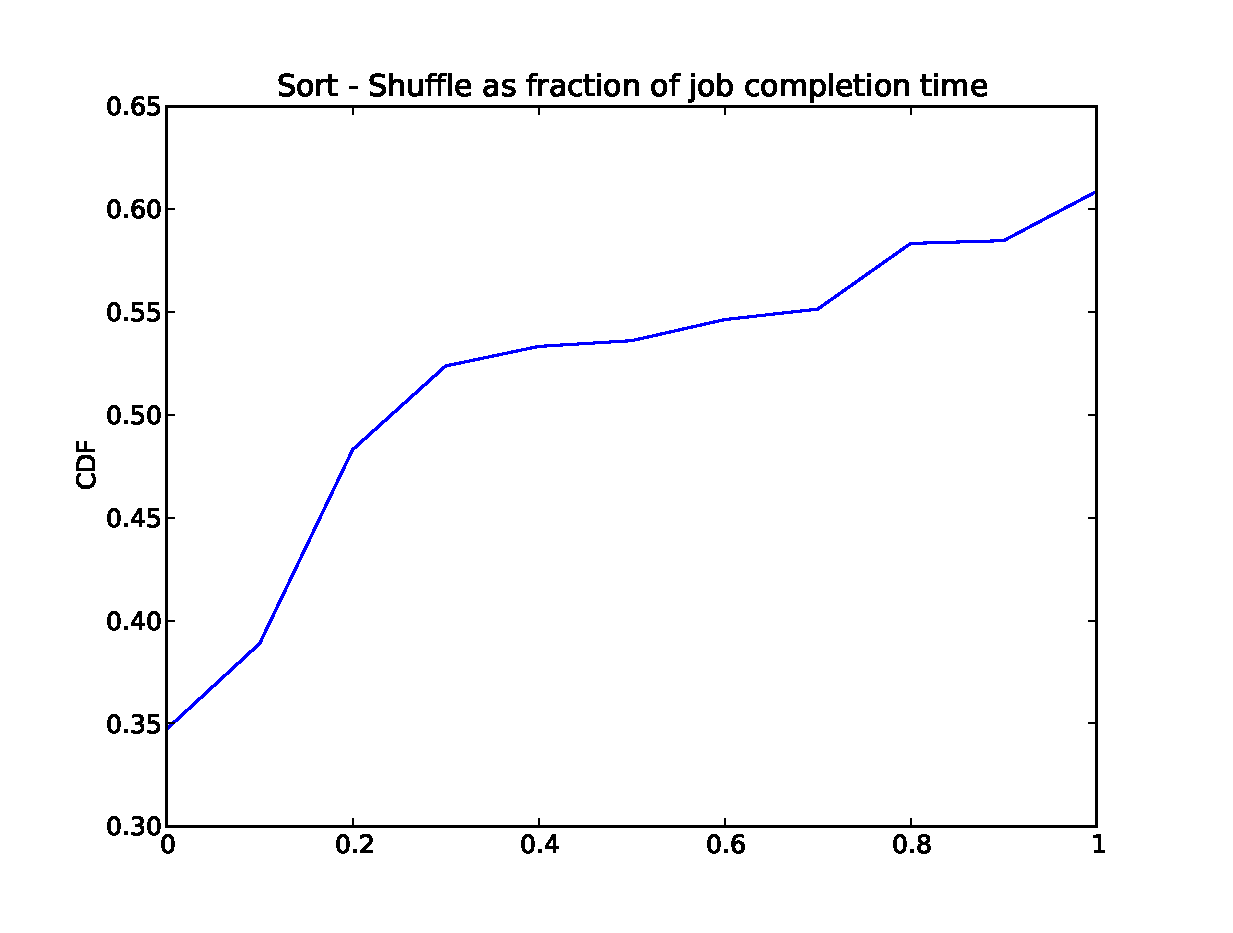
\includegraphics[width=0.8\textwidth]{sort_fraction.eps}
    \caption{Shuffle time as a fraction of execution time for Sort}
    \label{chap:introduction:fig:sort_fraction}
\end{figure}

It is important to highlight that some of these problems, stem at least in part
from the difference in traffic characteristics and scale between data centers
and other networks. In addition, unlike wide area network applications, there is
a tight coupling between an application's usage of network, compute, and storage
resources. In production data centers, due to the widely-varying mix of
applications, congestion in the network can last from 10s to 100s of
seconds~\cite{Kandula:2009:NDC}. Moreover, during high utilization periods, the
task failure rate of batch-processing systems increases, especially during the
\emph{reduce} phase of MapReduce-style applications, by a median value of 1.1x,
due to read failures over the network. In the worst case, this can halt the
entire job if subsequent tasks are dependent on the failed ones. Furthermore,
link utilization is highest in the core of the network, but most losses occur
towards the edge~\cite{Benson:2010:NTC}. Additionally, in some cases
over-provisioning the network is overkill and good performance can be achieved
by adding a few extra links at hotspot points~\cite{Kandula:2009:FTD}. Finally,
in commodity switches the buffer pool is shared by all interfaces. As a result,
if long flows hog the memory, queues can build up for the short flows.
In reaction, TCP reduces the window size by half. This leads to a large mismatch
between the input rate and the capacity of the link, leading to buffer
underflows and loss of throughput~\cite{Alizadeh:2010:DCT}. Overall, traffic
engineering in the data center is a complex task due to the wide variability in
flow duration, flow size, flow arrival time, and server
participation~\cite{Kandula:2009:NDC}: Standard TCP without any global knowledge
is suboptimal~\cite{Benson:2010:CFT}.

Another major shortcoming of TCP, which is manifest in the data center, is TCP
throughput collapse, or
\emph{incast}~\cite{Chen:2009:UTI,Vasudevan:2009:SEF,Wu:2010:IIC,Alizadeh:2010:DCT}.
This can cause overall application throughput to decrease by up to
90\%~\cite{Vasudevan:2009:SEF}. Typically, to handle incast, application-level
remedies are added which include varying the size of the packets so that a large
number of packets can fit the switch memory, and adding application-level jitter
to decorrelate the packet inter-arrival time. Both of these solutions are
suboptimal, as they either increase the number of packets, or add unnecessary
delay~\cite{Alizadeh:2010:DCT}. Finally, most applications operate in a
virtualized environment where a single host runs tens of virtual machines (VM).
This sharing of CPU by multiple VMs increases the latency experienced by each
VM, which can be orders of magnitude higher than the RTT between hosts inside a
data center~\cite{Gamage:2011:OFI,Kangarlou:2010:VIT}. This significantly slows
down the progress of TCP connections between different applications. So much so
that there are periods where TCP throughput can go down to
zero~\cite{Wang:2010:IVN}.

All of these problems have even prompted large-scale deployments to abandon TCP
altogether. For instance, Facebook~\cite{Facebook} now uses a custom UDP
transport. Some researchers have gone to the extent of suggesting that fixing
TCP is tantamount to ``saving the world''~\cite{Lyon:2008:TII}\footnote{Heat and
CO$_{2}$ emissions, and radioactive waste can be accounted to TCP's
inefficiency.}. For completeness, it is worth noting that TCP was designed as a
general transport mechanism for a wide area network (WAN)~\cite{Clark:1988:DPD}
and has experienced near universal adoption in environments as diverse as
satellites~\cite{Henderson:1999:TPF}. This is primarily due to TCP's ability to
provide reliability, congestion and flow control, and in-order packet delivery.
Moreover, its maturity makes it a ``kitchen sink'' solution for
developers~\cite{Vasudevan:2009:SEF}. Naturally, it has become the transport of
choice for the data center. But it is clear from the discussion above that TCP
is sub-optimal in a data center environment -- a fact agreed upon universally by
researchers. As a result, in recent years, a number of novel versions of TCP
have been
proposed~\cite{Alizadeh:2010:DCT,Wu:2010:IIC,Wilson:2011:BNL,Vasudevan:2009:SEF,Chen:2009:UTI}.
Unfortunately, most solutions are tied either to the underlying topology or the
structure and traffic mix of the data center: There is no one-size-fits-all
solution.

\section{Augmenting the Narrow-waist of the Data Center}
It should be clear from the discussion above that the data center communication
optimization space is wide due to the interplay of data center structure,
traffic patterns, and application requirements. Traffic engineering that
performs optimal routing in the data center requires global state, multi-path
routing, and the assumption of short-term predictability for
adaptation~\cite{Benson:2010:CFT,Benson:2011:MFG}. Further, data intensive
computing frameworks (DICF) work at the level of a \emph{transfer}, which is not
covered by existing solutions which operate at the flow or packet
level~\cite{Chowdhury:2011:MDT}. Put differently, stages between DICF are
dependent on bulk \emph{transfers} of data. These requirements suggest that
there needs to be a decoupling between data transfer policy and mechanism.
Therefore, in light of these requirements, this thesis proposes application and
network characteristics-centric data transfers. The same strategy when applied
at the network layer improves both application-level and network-level
performance~\cite{Abu-Libdeh:2010:SRF}. In addition to improving performance,
transport layer characteristics can also be chosen to improve energy
efficiency~\cite{Heller:2010:ESE} or security~\cite{bittau:the}. Adding power
constraints can greatly reduce the consumption footprint of today's data centers
where the network consumes 10-20\% of the total power~\cite{Greenberg:2008:CCR}.
Likewise, application traffic can transparently and
efficiently~\cite{bittau:the} be encrypted to ensure security in a multi-tenant
environment.

The rest of this document is structured as follows. \S\ref{chapter:background}
gives an overview of the cloud computing paradigm, data intensive computing
frameworks, and application models in the cloud. Related work is summarized in
\S\ref{chapter:relatedWork}. \S\ref{chapter:designImplementation} presents the
design and implementation of Mission Control. An evaluation of the network
patterns of existing systems and of Mission Control is given in
\S\ref{chapter:evaluation}. Finally, \S\ref{chapter:conclusion} concludes and
points to future work.

\chapter{Background}\label{chapter:background}
This section first gives an overview of cloud computing
(\S\ref{chapter:background:section:cloudComputing}), followed by an introduction
to data intensive computing frameworks
(\S\ref{chapter:background:section:dataIntensive}), and finally, a discussion on
consistency, replication, scalability, and reliability in the context of cloud
computing (\S\ref{chapter:background:section:consistency}).

\section{Cloud Computing}\label{chapter:background:section:cloudComputing}
Cloud computing is an all encompassing term for applications (services from the
point of view of the average user), software systems, and the hardware in
massive data centers~\cite{Armbrust:2009:ATC}. \emph{Public clouds} are used by
companies to provide utility computing in which software (SaaS), infrastructure
(IaaS), and platform (PaaS) can be a service. Similarly, organizations and
companies also maintain \emph{Private clouds} which are used internally for data
processing and storage. In the cloud computing model, users can buy \emph{X} as
a service (XaaS), where X can be software, infrastructure, and platform and
elastically increase or decrease required resources based on dynamic
requirements. This allows the user to focus on application design without having
to worry about system or network administration. The ascent of cloud computing
has been fuelled by the rise of ``Big Data'' and in turn, data intensive
computing. The Cloud has become the ideal platform to store and analyze massive
datasets generated by applications as diverse as satellite imagery and web
indexing. Batch processing systems, such as MapReduce~\cite{Dean:2004:MSD}, are
in turn used to compute user queries over these datasets. Finally, users can
leverage the ``cost associativity''\footnote{Using a large number of computers
for a short time costs the same amount as using a small number for a long time.}
of the Cloud and the parallelism in the application to speed up the job
completion time. Data intensive computing frameworks are the subject of the next
section.

\section{Data Intensive
Computing}\label{chapter:background:section:dataIntensive}
Google's MapReduce~\cite{Dean:2004:MSD} and its open source counterpart, Hadoop
~\cite{hadoop}, are at the forefront of data intensive computing. MapReduce is a
programming model and execution engine for performing large-scale computation on
a cluster of commodity machines. It abstracts work division, communication, and
fault tolerance beneath a two function API. The user only needs to specify one
\emph{map} and one \emph{reduce} function, while the framework takes care of the
rest. The architecture consists of a master node and a set of worker nodes.
The master node schedules shards of the input dataset -- stored on a distributed
filesystem -- on the worker nodes. The entire execution is two-phased: first the
map function is applied to all chunks of input data by the worker nodes,
followed by the application of the reduce function to the output of the mappers.
The framework operates on key-value pairs. The intermediate key-value pairs,
obtained after the map phase, are \emph{shuffled} to a set of reduce workers
based on hash partitioning. The framework also has several optimizations such
as: (1) Locality: input data is assigned on the basis of locality, (2)
Fault-tolerance: failed tasks are simply rescheduled, and (3) Speculative
re-execution: slow executing tasks are speculatively re-executed on other nodes
to improve the job completion time.

One major shortcoming of MapReduce is that it is strictly a two-phase
architecture, as a result of which, it cannot easily express multi-phase
SQL-like queries. Implementing these queries is awkward in the MapReduce
paradigm as they constitute multiple MapReduce jobs, requiring external
operators to merge the output~\cite{Yang:2007:MSR}. Additionally, the framework
is also handicapped by its single input, single output restriction. These
shortcomings are addressed by Microsoft's Dryad system~\cite{Isard:2007:DDD}.
Dryad is a general purpose framework that supports the processing of algorithms
with directed cyclic graph (DAG) flows. Like MapReduce, the framework abstracts
work scheduling, data partitioning, fault tolerance, and communication beneath a
data-flow execution engine. To this end, the developer only needs to (a)
construct a DAG of processing using provided primitives, and (b) provide a
binary executable for nodes in the DAG. Each vertex in the graph represents the
execution of some operation over its input data, while the edges between the
vertices represent the communication patterns. The framework automatically
schedules each vertex to a machine/core and sets up the communication channels.
It is important to highlight that unlike MapReduce, Dryad vertices can have
multiple inputs and outputs depending on the programming semantics. Finally,
developers can easily use high-level languages to restrict the programming
interface for a particular domain.

While MapReduce and Dryad are efficient at processing a rich set of applications
with sequential flow, they fall short of supporting iterative and recursive
applications~\cite{Bu:2010:HEI,Zaharia:2010:SCC}. In addition, these
applications, such as \emph{k}-means clustering, PageRank, etc., require a more
expressive language to define their flow. These problems are addressed by
CIEL~\cite{Murray:2011:CUE} which includes two components: (1) A scripting
language, \emph{Skywriting}~\cite{Murray:2010:SCS}, and (2) A distributed
execution engine. Skywriting is a Turing-complete language that can be used to
express data-dependent control flow. It provides primitives to loop over
expressions or call them recursively. In addition, scripting primitives can be
used to spawn and execute tasks, and de-reference data (reminiscent of pointers
in C/C++). Further, it provides library functions to express the flow of other
frameworks such as MapReduce, as CIEL subsumes both MapReduce and Dryad.
Architecturally, CIEL is similar to MapReduce and Dryad, in that it also has a
single master and several worker nodes, with the former in charge of computation
state, and the latter in charge of the actual computation.
CIEL relies on three primitives -- objects, references, and tasks -- for
defining dynamic task graphs. Specifically, objects are data sequences that are
used for input and are generated as output. Objects which have not been fully
computed yet, can be used as references. Further, tasks are the unit of
computation and scheduling. Tasks use programmatic code, or binaries to execute
over all their dependencies. Moreover, tasks can either compute all of their
output objects, or alternatively, spawn other tasks to do so. Tasks can be
executed in either \emph{eager}, or \emph{lazy} fashion, with the latter being
the default strategy. Finally, CIEL uses a number of optimizations to improve
performance such as deterministic naming, and streaming.
Figure~\ref{chap:intro:fig:frameworks} highlights the major differences between
the three frameworks.

\begin{figure}[h!]
        \begin{subfigure}[b]{0.4\textwidth}
                \centering
                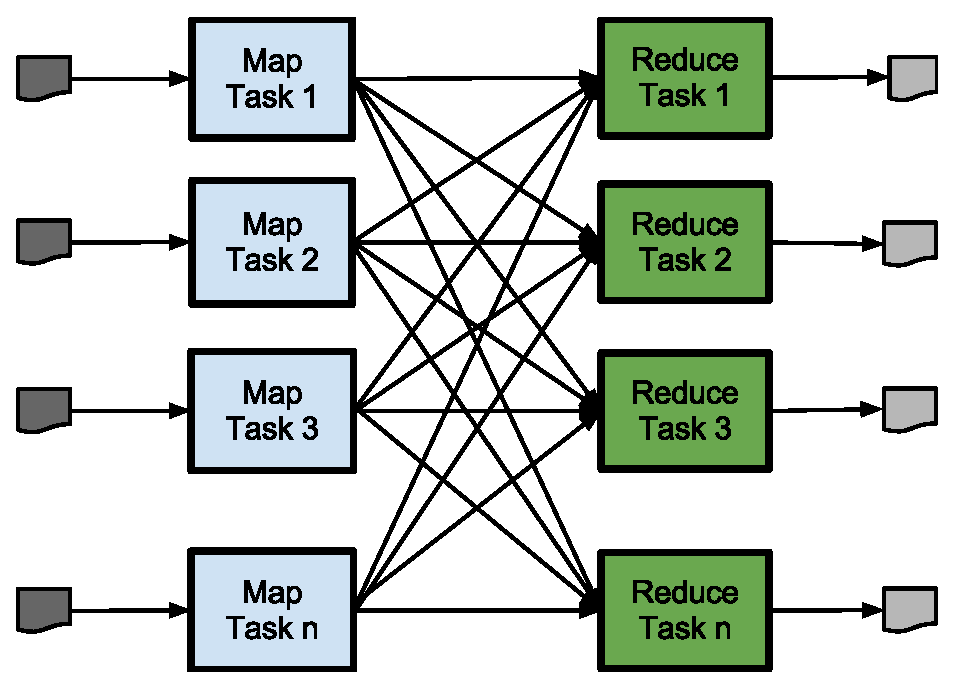
\includegraphics[width=\textwidth]{MapReduce.eps}
                \caption{MapReduce has
        two stages with single input and single output.}
                \label{fig:mapreduce}
        \end{subfigure}%
        \hspace{0.1pt}
        \begin{subfigure}[b]{0.5\textwidth}
                \centering
                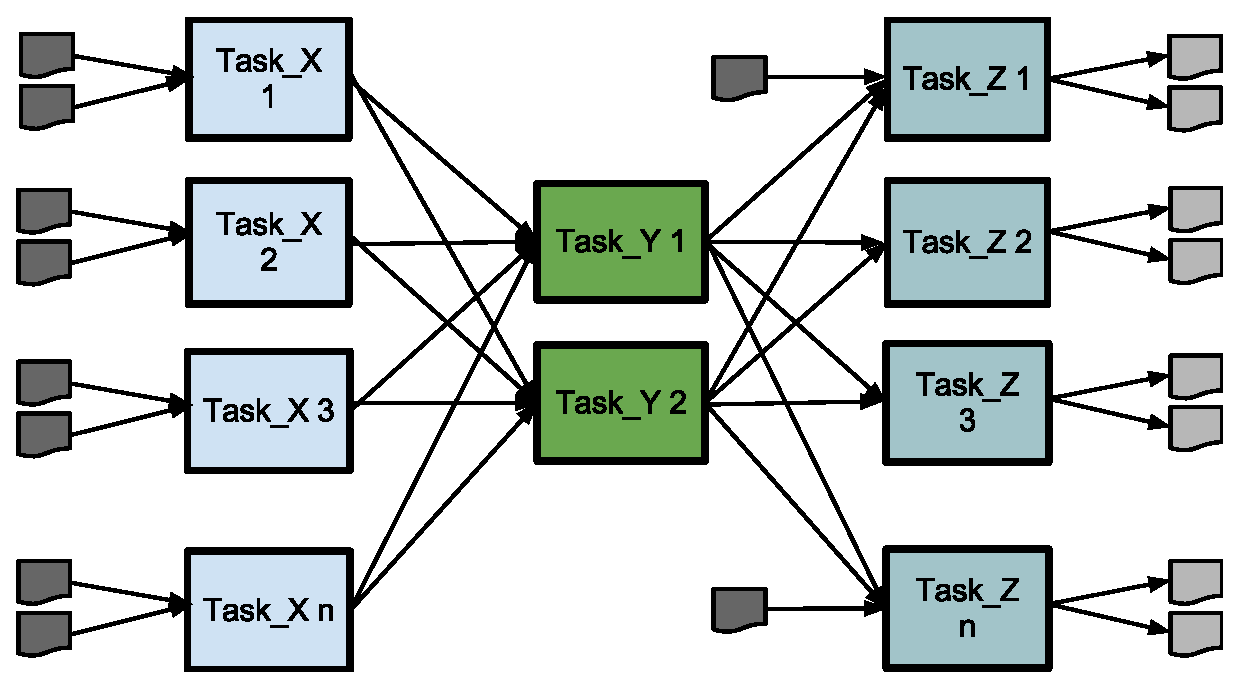
\includegraphics[width=\textwidth]{Dryad.eps}
                \caption{Dryad execution can
        consist of multiple stages with multiple input and multiple output.}
                \label{fig:dryad}
        \end{subfigure}
        \vspace{0.1pt}
        \begin{subfigure}[b]{0.8\textwidth}
                \centering
                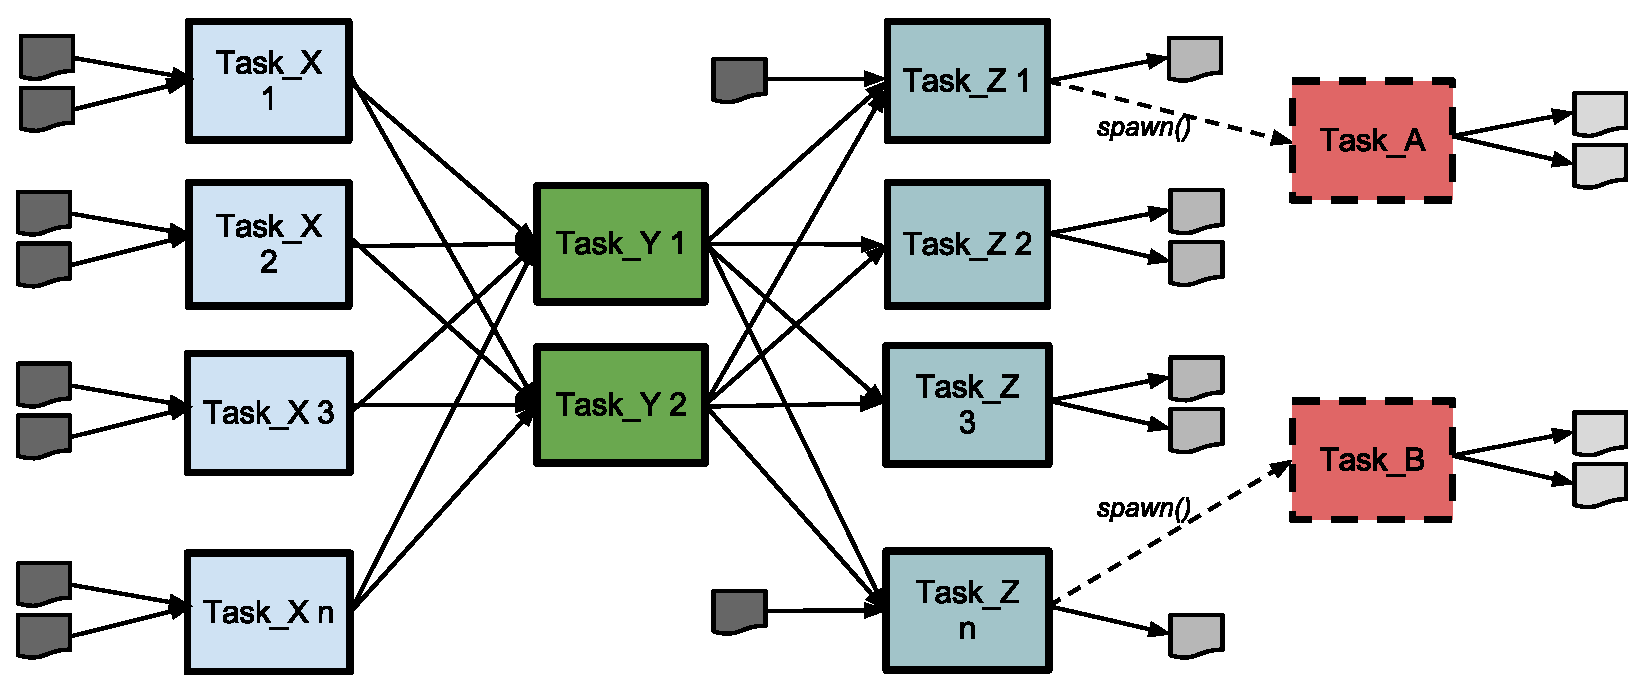
\includegraphics[width=\textwidth]{CIEL.eps}
                \caption{CIEL
        execution, which subsumes MapReduce and Dryad, can consist of multiple
        stages with multiple input and multiple output and tasks can dynamically
        spawn other tasks as well.}
                \label{fig:ciel}
        \end{subfigure}
        \caption{Overview of data intensive computing frameworks.}
        \label{chap:intro:fig:frameworks}
\end{figure}

There are also high-level
languages~\cite{Olston:2008:PLN,Pike:2005:IDP,Murray:2010:SCS,Yu:2008:DSG} which
allow users to write applications which are transparently translated into a
data-flow plan, and then scheduled on top of the underlying framework. In
addition, there is a rich body of work which aims to reduce the turn-around time
of these systems~\cite{Zaharia:2010:DSS,Isard:2009:QFS,Zaharia:2008:IMP}. While
these proposals have been successful in improving scheduling and fairness, the
network utilization of these batch-processing systems has largely been ignored.

As mentioned earlier, these frameworks operate over large amounts of data inside
environments which are error-prone. Therefore, they have to make trade-offs
between consistency, replication, scalability, and reliability. These issues are
discussed in the next section.

\section{Consistency, Replication, Scalability, and Reliability in the
Cloud}\label{chapter:background:section:consistency}
It is a well-known principle that it is hard to build distributed systems which
are consistent, available, reliable, and scalable. In fact, according to
Brewer's CAP theorem, it is impossible to build a distributed system which has
consistency (all nodes see the same data), availability (the service is always
accessible), and partition tolerance (the services can tolerate the loss of
nodes/data) at the same time~\cite{Brewer:2000:TRD,Gilbert:2002:BCF}. Developers
have to sacrifice one of the three. Due to the failure-prone, commodity
infrastructure used to build distributed systems today, partition tolerance is a
given. Therefore, systems have to make a choice between consistency and
availability~\cite{Vogels:2009:EC}. Most cloud applications today, such as
Amazon's Dynamo~\cite{DeCandia:2007:DAH} focus on availability, resulting in
weak consistency or \emph{eventual consistency}. This basically available, soft
state, eventually consistent (BASE)~\cite{Pritchett:2008:BAA} model enables
applications to function even in the face of partial failure. To this end,
applications operate on local (possibly stale) replicas, while the underlying
system asynchronously applies updates to replicas.

One way to implement replication updates is through \emph{virtual
synchrony}~\cite{Birman:1987:EVS}. In this model, processes are organized into
dynamic \emph{process groups}, and messages are exchanged between groups, not
individual processes, with ordering guarantees. From the perspective of the
application, all changes to the shared data appear to be synchronous. As process
groups can have names, they can be treated as topics in a publish-subscribe
system~\cite{Birman:2010:AHO}. In addition, processes within the group are
informed if group membership changes to ensure a consistent view of group
membership across all members. Whenever a new member joins a process group, the
current state is checkpointed and sent to the newly joined member to initialize
its group replica in one atomic operation. Processes can also send multicast
events to groups with ordering guarantees.

These issues are important for a distributed system such as Mission Control, as
performance can be dependent on the durability and consistency of control
traffic. As mentioned earlier, the traffic matrix in a data center can change in
a matter of seconds, therefore, Mission Control needs to be able to respond in a
timely fashion.

\chapter{Related Work}\label{chapter:relatedWork}
This section presents relevant related work on data center networking in general
and also specific to data intensive computing. Specifically, we summarize recent
work in novel data center topologies, L2-, L3-, and L4-layer protocols,
schedulers, resource allocators, traffic reduction, and rate controllers. 

\section{Topologies}
Data intensive computing frameworks such as MapReduce require full-bisection
bandwidth during the data shuffle phase. Unfortunately, a regular 2/3-layer tree
topology is unable to cater to this need as links up the tree hierarchy are
shared and hence, become a bottleneck. To remedy this, a number of novel
topologies have recently been proposed.

Al-Fares et al.~\cite{Al-Fares:2008:SCD} present a data center architecture
using a fat-tree topology which aims to support full-bisection bandwidth. A
\emph{k}-aray fat-tree enables each host and switch to have redundant links. IP
addresses are assigned in the network based on the location of the element in
the topology. To achieve even load balancing, a two-level routing table is
employed. Further, a central route control statically generates all routing
tables and loads them into switches. In addition, the architecture also enables
flow classification and scheduling to minimize overlap between flows. Finally, a
failure broadcast protocol is used to enable switches to route around failures.
VL2~\cite{Greenberg:2009:VSF} also uses a fat-tree topology but requires no
changes to the underlying L2 fabric. It uses two different addressing schemes to
simplify virtual machine migration. Interfaces and switches use
location-specific addresses while applications use application-specific
addresses. The mapping between these two schemes is maintained by a replicated
directory service. To spread traffic over the multiple links, VL2 uses both
valiant load balancing (VLB) and equal-cost multi-path routing (ECMP).

In contrast to fat-tree and VL2, DCell~\cite{Guo:2008:DSF} is a recursive,
server-centric architecture. Each server is connected to other servers directly
and through a small number of switches. DCells form a fully-connected graph and
can be assembled together to form high-level DCells. Servers in DCells are
identified by their position in the structure. Further, the architecture uses a
fault-tolerant single-path routing algorithm that exploits the recursive
structure of the topology. A related architecture, BCube~\cite{Guo:2009:BHP}, is
similar in structure but targets modular data
centers~\cite{Vishwanath:2009:MDC}. Switches in BCube only connect servers,
while servers themselves relay their traffic. Servers are addressed using an
array based on their position, as a result neighbouring servers only differ by a
single digit in the array. This information is used by source servers to encode
routing information in the packet headers, which are in turn, used by servers
for packet forwarding.

Another radical architecture is CamCube, which proposes a 3D torus topology in
which each server is directly connected to a small set of other servers,
inspired by structured overlays~\cite{Abu-Libdeh:2010:SRF}. This scheme places
each server into a 3D wrapped coordinate space and its position (\emph{x,y,z})
in the space represents its address. As a result, the physical and virtual
topology of the network is the same and applications can infer their location
through an API which exposes coordinate space information and allows one-hop
Ethernet packets. Thus, applications can implement their own routing strategies.

One problem that plagues these topologies is of incremental expansion. As a
result of their rigid, well-defined structure, incremental expansion can only be
done if the structure is preserved. Jellyfish~\cite{Singla:2011:JND} addresses
this problem by constructing a random graph topology. Random graphs achieve low
diameter and high bisection bandwidth while allowing incremental expansion with
any number of nodes. At the same time, Jellyfish can enable full-bisection
bandwidth with a lower switch count than a fat-tree.

Finally, these topologies have also spawned a number of systems to improve their
management and construction. Alias~\cite{Walraed-Sullivan:2011} and
DAC~\cite{Chen:2010:GAA} can be used to automatically assign addresses to these
topologies. Perseus~\cite{Mudigonda:2011:TFC} is a framework that enables
designers to choose an optimum data center design based on bandwidth, cost,
application requirements, etc. The framework currently supports fat-tree and
HyperX topologies. Specifically, user requirements and chosen topologies are
given as input to Perseus which then generates a design with a candidate
topology, optimized cabling, cost, and a visualization of the structure.

Although, these topologies expose full bisection bandwidth, in practice due to
multi-tenancy~\cite{Costa:2012:CEI}, and TCP's inefficiency in (a) moving away
from congested links, and (b) exploiting multiple links~\cite{Raiciu:2011:IDP},
applications do not experience the full benefit. In addition, these topologies
also increase the overall cost and wiring complexity. In data centers which
already have these topologies, Mission Control can be used to exploit their
multiple links. 

\section{Ethernet Fabrics}
Ethernet also faces a number of scalability challenges in a data center
environment. 

SPAIN~\cite{Mudigonda:2010:SCD} is an Ethernet fabric that implements forwarding
along multiple paths connected by commodity switches and arbitrary topologies.
Specifically, it overcomes the single spanning restriction of the Spanning Tree
Protocol (STP) by making use of multiple spanning trees which are calculated
offline. In topologies with multiple paths, each spanning tree is organized into
a separate VLAN to exploit path redundancy. In addition, it also minimizes the
overhead of packet flooding and host broadcasts.
NetLord~\cite{Mudigonda:2011:NSM} is a related system which enables flexibility
in choosing VM addresses. To this end, it implements IP encapsulation for custom
L2 packets and uses SPAIN as the underlying fabric. This enables NetLord to
scale to a large number of tenants and VMs. It also uses a custom push-based ARP
protocol to keep location information consistent. Similarly,
Portland~\cite{NiranjanMysore:2009:PSF} is a layer 2 routing and forwarding
fabric that uses topological information to assign end-hosts hierarchical
pseudo-MAC (PMAC) addresses. It employs a centralized directory service to map
PMAC onto physical MAC addresses. All routing and forwarding takes place using
PMAC prefixes while the end-hosts only see MAC addresses. In addition, the
centralized directory service eliminates the need for broadcast based ARP and
DHCP. Finally, end-hosts are modified to spread load over the available paths.
Vattikonda et al. explore a new point in the design space by dispensing with TCP
altogether and replacing it with a time-division multiple access (TDMA) MAC
layer~\cite{Vattikonda:2012:PTD}. To this end, they employ centralized
scheduling to give communicating end-hosts exclusive access to links. This
exclusive assignment of link bandwidth and switch buffer space automatically
mitigates in-network queuing and congestion. All of these proposals work at
layer 2 and are as such, complementary to our work.

\section{Global Schedulers and Resource Allocators}
To enable applications to make use of multiple paths in the network, a number of
schedulers have also been proposed. One such scheduler is
Hedera~\cite{Al-Fares:2010:HDF} which uses flow information from Openflow
switches to compute non-conflicting paths for flows, which are in turn pushed
back to the switches. This enables the network to maximize bisection bandwidth.
It provides a number of algorithms for choosing optimum paths. Similarly,
DevoFlow~\cite{Curtis:2011:DSF} is a modification of the Openflow architecture
that tries to handle most flows in the data plane to achieve scalability. Hence,
Hedera-like schedulers only need to deal with \emph{interesting} flows.

MicroTE~\cite{Benson:2011:MFG} is a traffic engineering system that adapts to
variation in network traffic at the granularity of a second. It consists of a
central controller that creates a global view of traffic demands and coordinates
scheduling using Openflow. To this end, it differentiates between predictable
traffic and non-predictable traffic. For the former, it computes routes based on
some global objective to achieve optimum routing. The leftover routes are then
used to stripe unpredictable traffic using weighted equal-cost multi-path
routing (ECMP).

A recent system, Orchestra~\cite{Chowdhury:2011:MDT}, works at the application
layer to enable intra- and inter-transfer control of two communication patterns,
which lie at the heart of batch processing systems such as MapReduce:
\emph{shuffles}, and \emph{broadcasts}. For the former, it uses weighted flow
assignment (WFA) enabled by an appropriate number of multiple TCP connections
and TCP's AIMD fair sharing while for the latter it leverages a BitTorrent-like
algorithm. Architecturally, it is a centralized application layer controller for
both intra- and inter-transfer communication. The former is managed by one or
more Transfer Controllers (TCs) while the latter is managed by an Inter-transfer
Controller (ITC). The TC continuously monitors the transfer and updates the set
of sources associated with each destination. Specifically, the TC manages the
transfer at the granularity of flows, by choosing how many concurrent flows to
open from each node, which destinations to open them to, and when to move each
chunk of data. While the results from Orchestra are promising, it is still
suboptimal due to its reliance on TCP. In addition, frameworks like Dryad
support TCP pipes, and shared memory FIFO for communication in addition to
transfer of files over the network, while Orchestra only considers the last of
these.

In contrast to all of these systems, Mission Control uses the diversity in
transport protocols to achieve optimum routing and congestion control. At the
same time, the architecture of Mission Control is inspired by the architecture
of Orchestra.

\section{Transport Protocols}
In this section we enumerate transport protocols which address some of
TCP's shortcomings.

Deadline-Driven Delivery (D$^3$)~\cite{Wilson:2011:BNL} is a data
center-specific version of TCP that targets applications with distributed
workflow and latency targets. These applications associate a deadline with each
network flow and the flow is only useful if the deadline is met\footnote{TCP on
the other hand tries to achieve global fairness and maximize throughput while
remaining agnostic to any flow-specific deadline.}. To this end, applications
expose flow deadline and size information which is exploited by end hosts to
request rates from routers along the data path. Routers only maintain aggregate
counters and thus, do not maintain any per-flow state. As a result, they are
able to allocate sending rates to flows in order for as many deadlines to be met
as possible. On the downside, D$^3$ requires changes to applications, end-hosts,
and network elements. For data centers with customizable network elements,
Mission Control can use D$^3$ for applications that expose explicit deadline
information.

Data Center TCP (DCTCP)~\cite{Alizadeh:2010:DCT} uses Explicit Congestion
Notifications (ECN) from switches to perform active queue management-based
congestion control. Specifically, it uses the congestion experienced flag in
packets---set by switches whenever the buffer occupancy exceeds a small
threshold---to reduce the size of the window based on a fraction of the marked
packets. This enables DCTCP to react quickly to queue buildup and avoid buffer
pressure. DCTCP can only work in a network with ECN-compatible switches.
Therefore, Mission Control enables DCTCP if it detects that switches in the
network support ECN. A spin-off architecture is HULL~\cite{Alizadeh:2012:LIM},
high-bandwidth ultra-low latency, that aims to make a trade-off between
bandwidth and latency for low-latency applications in a shared environment. To
this end, it reduces network buffering by replacing queue occupancy-based
congestion control with link utilization. It makes use of \emph{phantom queues}
which give the illusion of draining a link at less than its actual rate.
End-hosts employing DCTCP experience reduced transmission rates based on ECN
from these phantom queues. This enables the overall network to trade bandwidth
for latency.

Structured Stream Transport (SST)~\cite{Ford:2007:SSN} finds the middle-ground
between stream and datagram transmission. It implements a hierarchical and
hereditary stream structure which allows applications to create substreams from
existing streams without incurring startup and tear-down delay. Substreams
operate independently with their own data transfer and flow control. To ensure
inter-stream fairness, substreams share congestion control. Moreover,
``ephemeral streams'' can be used to enable datagram transmission. Finally,
applications can prioritize their streams on the fly depending on runtime
requirements. Mission Control can use SST to enable MapReduce-like systems to
prioritize their data transfers, by opening multiple substreams, and to send
lightweight control traffic using ephemeral streams.

Raiciu et al.\cite{Raiciu:2010:DCN} argue that current data center architectures
use random load balancing (RLB) to balance load across multiple paths. RLB is
unable to achieve full bisectional bandwidth because certain flows always
traverse the same path. This creates hotspots in the topology, where certain
links are oversubscribed and some are under/un-subscribed. Global flow
controllers fail in this regard too as they are unable to scale with the number
of flows. To remedy this, they propose the use of multi-path TCP (MPTCP) to
establish multiple subflows over different paths between a pair of end-hosts.
The key point is that these subflows operate under a single TCP connection. They
argue that this ensures fairness as the fraction of the total congestion window
for each flow is determined by its speed, i.e. the faster a flow is, the steeper
the slope of its additive increase. This will also move traffic away from the
most congested paths. MPTCP is supposed by Mission Control in multi-path
networks.

\subsection{Incast}
A number of proposals have also tried to tackle incast. 

Vasudevan et al.~\cite{Vasudevan:2009:SEF} propose that we increase the
granularity of kernel timers to enable microsecond granularity RTT estimation,
which is in turn used to set the RTO. They show that reducing the RTO can
increase the goodput of simultaneous connections and hence negate incast.
Furthermore, making retransmissions random can also increase the goodput by
stopping multiple flows from timing out, backing off, and retransmitting
simultaneously. The takeaway lesson is that to avoid incast in low-latency data
center networks, RTOs should be on the same scale as network latency. Chen et
al.~\cite{Chen:2009:UTI} complement the analysis of the previous work by
defining an analytical model for incast. This model shows that goodput is
affected by both the minimum RTO timer value and the inter-packet wait time.
Unlike these two solutions which focus on post hoc recovery,
ICTCP~\cite{Wu:2010:IIC} aims to avoid packet losses before incast
manifestation. To this end, ICTCP implements a window-based congestion control
algorithm at the receiver side. Specifically, the available bandwidth at the
receiver is used as a trigger to perform congestion control. The frequency of
this control changes dynamically based on the queueing delay and is larger than
one RTT. Connection throughput is only throttled to avoid incast, not to
decrease application goodput. 

\section{Data Center Traffic Analysis}
Kandula et al.~\cite{Kandula:2009:NDC} present an analysis of the traffic of a
1500 server data center. They use lightweight measurements at end-hosts in
conjunction with application level data to note the cause and effect of network
incidents. The target applications have a work-seeks-bandwidth and
scatter-gather pattern. Their analysis shows that most traffic is exchanged
within a rack and on average, a server communicates with two servers within its
rack and four outside the rack. With respect to congestion, their study shows
that highly utilized links are prevalent and congestion can last from 10s of
seconds to 100s. In addition, most periods of congestion are short lived.
Further, during periods of congestion there is an increase in the number of
worker failures. Finally, traffic patterns change both frequently and quickly
over time. Following in the footsteps of Kandula et al., Benson et
al.~\cite{Benson:2009:UDC}, present SNMP data from 19 data centers. Their
analysis shows that traffic load is high in the core and decreases towards the
edge. At the same time, link loses are higher near the edge and decrease towards
the core. In addition, a small fraction of the links account for most losses.
This observation shows that traffic can be routed along alternate routes to
avoid congestion. Finally, traffic is bursty in nature and packet inter-arrival
times during spike periods follow a lognormal distribution. In a follow-up
paper, Benson et al.~\cite{Benson:2010:NTC} augment their previous work by
studying different classes of data centers. These include, university campus,
private enterprise, and cloud data centers. In this work, they examine the
variation in link utilization and the magnitude of losses as well as the nature
of hotspots. Their measurements show that for cloud data centers, 80\% of the
traffic stays within the rack and the number of highly utilized core links never
exceeds 25\% of the total links.

We use the insight provided by these studies to keep the design of Mission
Control generic enough to cater to the needs of these widely-varying traffic
patterns.

\section{Reducing Network Traffic}
Another point in the design space is to reduce the amount of traffic that is
transferred across the network by MapReduce-like
systems~\cite{Costa:2012:CEI,Yu:2009:DAD}. This can be done either across
different levels in the cluster topology~\cite{Yu:2009:DAD}, or made a function
of the network itself as in Camdoop~\cite{Costa:2012:CEI}. On the downside,
performing rack-level aggregation can saturate the ingress link to the
aggregating server~\cite{Yu:2009:DAD}. This \emph{distributed combiner} approach
is most effective for MapReduce functions which are commutative and
associative~\cite{Dean:2004:MSD}. In the same vein, SUDO~\cite{Zhang:2012:ODS}
leverages the functional and data-partition properties of user-defined functions
in MapReduce-like systems to enable various optimizations. This enables the
framework to avoid unnecessary data-shuffling steps and reduce disk and network
I/O. While these frameworks reduce the amount of data transferred across the
network, they still rely on standard TCP, inheriting its flaws.

\section{Wireless and Optical Networks}
Another line of work has argued that providing full-bisection links throughout
the network is overkill as only a few hotspots exist in actual data
centers~\cite{{Halperin:2011:ADC,Kandula:2009:FTD}}. The high cost and technical
challenges of newer topologies can be avoided by provisioning the network for
the average case and avoiding hotspots by adding additional links on the fly.
The key challenge is to choose the placement and duration of \emph{flyways}.
In these proposals, flyways are constructed using Multi-Gigabit wireless links,
controlled by a centralized scheduler that decides the temporal and spatial
placement of wireless links based on observed traffic. On major shortcoming of
this approach is that in cases where the traffic has high churn, the controller
would fail to respond quickly.

Likewise, c-Through~\cite{Wang:2010:CPO} and Helios~\cite{Farrington:2010:HHE}
consider using hybrid packet and circuit switched networks in order to use
optical links to address hotspots. c-Through connects racks using optical
circuit-switched links based on traffic demand. Network isolation is ensured by
using a separate VLAN for the optical and electrical rack links. End-hosts are
used for traffic statistics collection while a central manager, connected to the
optical switch, is used to manage configuration. In contrast,
Helios~\cite{Farrington:2010:HHE} targets modular data
centers~\cite{Vishwanath:2009:MDC}. It uses flow counters in switches to
calculate the traffic matrix and in turn, uses that information to work out a
topology to maximize throughput. Finally, OSA~\cite{Chen:2012:OSA} is a
clean-slate all-optical network which can alter its topology and link capacities
based on the traffic demand.

While we do not consider wireless and optical links in this work, Mission
Control is flexible enough to support both. For example, Mission Control
maintains a global view of the network, therefore it can choose flyways or
optical paths for hotspots, if required.

\section{Virtualization and Rate Limiting}
To take advantage of economies of scale and achieve optimum resource
utilization, most data centers are virtualized. As a result, resources are
shared amongst the tenants, which can lead to contention and other undesired
behaviour.

Due to VM consolidation, the RTT of TCP connections to VMs increases
significantly, causing the latency of connections to go up. vSnoop is a system
that allows the driver domain of a host to send an acknowledgement on behalf of
the VMs~\cite{Kangarlou:2010:VIT}. It snoops on all VM traffic and maintains
per-flow state for each TCP connection which it then uses to enable early
acknowledgement of packets. The same problem afflicts the transmit path as well,
as TCP acknowledgements can get delayed, causing the TCP congestion window to
grow more slowly. To mitigate this, vFlood is another extension that offloads
congestion control to the driver domain, which allows the buffering of a high
number of packets~\cite{Gamage:2011:OFI}. Regardless of the transport protocol,
Mission Control can delegate congestion control to the driver domain in
virtualized environments.

Another related body of work deals with ensuring bandwidth fairness among
virtual machines and tenants in the data center. Seawall~\cite{Shieh:2010:SPI}
uses hypervisor-based rate limiting in conjunction with IP layer feedback
signals from the network to regulate egress traffic. Standard rate control
algorithms, such as TCP, TCP friendly rate control (TFRC), or quantized
congestion notification (QCN) are used to implement rate limiting. On the
downside, as Seawall is VM-centric, it does not divide the link bandwidth among
tenants using the link, but among the total number of VMs sending traffic
through that link. Therefore, tenants with a large number of VMs unfairly get a
large share in bandwidth. Similarly, Gatekeeper~\cite{Rodrigues:2011:GSB} works
at the virtualization layer of end-hosts to ensure bandwidth fairness. It
achieves scalability by using a point-to-point protocol and maintains minimum
data center-wide control state. Maximum and minimum rate is set for both ingress
and egress traffic at the vNIC level and scheduled using a weighted fair
scheduler. In addition, ingress and egress traffic is monitored and if limits
are exceeded, a feedback message with an explicit rate is sent to all VMs
involved in the traffic. Likewise, SecondNet~\cite{Guo:2010:SDC} uses a
\emph{virtual data center} (VDC) abstraction for resource allocation. It allows
the assignment of a set of VMs with computation, storage, and bandwidth
guarantees. Architecturally, a central manager is in charge of all resources
while virtual-to-physical mappings and network state is controlled by the source
hypervisors. While SecondNet can guarantee end-to-end bandwidth, it can only be
used if the bandwidth requirements are known a priori. Choosing an exact
bandwidth is non-trivial for most applications as bandwidth is a function of
their communication pattern. Oktupus~\cite{Ballani:2011:TPD} is a resource
allocator that uses ``virtual networks'' as an abstraction to expose to users.
This allows the cloud provider to decouple the virtual network and the
underlying physical network. As a result, there is a trade-off between
application goals for performance and provider goals for optimum utilization of
resources. For all-to-all communication, such as MapReduce traffic, a
\emph{virtual cluster} is employed which provides the illusion of all virtual
machines being connected to the same non-oversubscribed virtual switch.  For
applications with a local traffic pattern, a \emph{virtual oversubscribed
cluster} is employed which emulates an oversubscribed two-tier cluster.
Specifically, Oktupus uses physical network topology, machine usage, etc., to
allocate physical machines to users. In addition, explicit bandwidth
rate-limiting at the end hosts is employed to control bandwidth.

In this work we do not explicitly tackle VM rate limiting, but Mission Control
as an architecture can be used to rate limit ingress and egress links at the
application layer by controlling the transport schedule.

\section{Energy Efficiency and Security}
In addition to performance and fairness, energy efficiency and security are of
great important in the data center as well. 

ElasticTree is a system that dynamically alters the power consumption of
networking elements inside a data center based on the current
traffic~\cite{Heller:2010:ESE}. It consists of an optimizer, routing control,
and power control. Based on the topology, traffic matrix, and other inputs, the
optimizer computes an optimum power network subnet which is in turn fed to the
power control and the routing control. The former toggles the power state of
network elements, and the latter chooses paths for each flow. The optimizer
provides a number of strategies which make a trade-off between scalability and
optimality. ElasticTree can be used in conjunction with Mission Control to
choose a suitable underlying transport protocol. For example, the performance of
TCP is adversely affected if there is packet reordering due to splitting a
single flow across multiple links by ElasticTree.

TCPcrypt is a backwards compatible enhancement to TCP that aims to efficiently
and transparently provide encrypted communication to
applications~\cite{bittau:the}. To this end, it uses a custom key exchange
protocol that leverages the TCP options field. Like SSL, to reduce the cost of
connection setup for short-lived flows, it enables cryptographic state from one
TCP connection to bootstrap subsequent ones. Even for legacy applications, it
protects against passive eavesdropping. Additionally, TCPcrypt protects the
integrity of TCP sessions, and defends against attacks that change their state
or affect their performance.
Finally, applications can also be made aware of the presence of TCPcrypt to
negate redundant encryption. We use TCPcrypt as a secure transport protocol
option in Mission Control.

In summary, novel data center topologies in practice do no achieve
full-bisection bandwidth due to their reliance on TCP. In fact, in some cases
full-bisection bandwidth is overkill and the needs of most applications can be
satisfied by using a few additional links. Extensions to Ethernet can address
its scalability problems in the data center but the transport is still at the
mercy of TCP. In addition, global schedulers can take advantage of multiple
paths to improve performance but they either use TCP or ECMP which are by nature
suboptimal in the data center. Moreover, novel transport protocols only work in
specific environments for a limited number of traffic patterns. Furthermore,
aggressive use of \emph{combiners} can only reduce traffic to a certain extent.
Finally, rate limiters expect users to know the bandwidth requirements of their
applications beforehand. This is impractical as the prediction of network
traffic is non-trivial and application requirements dynamically change over the
course of their execution. Mission Control addresses the shortcomings of all of
these systems by enabling diversity in both transport semantics and scheduling.

\chapter{Design and Implementation}\label{chapter:designImplementation}
In this section, we present the design and implementation of Mission Control.

We first enumerate a set of goals for Mission Control:
\begin{enumerate}
  \item Mission Control should work out of the box. Therefore, it should require
  no changes to network infrastructure.
  \item There is no ``one-size-fits-all'' transport for the data center.
  Accordingly, Mission Control should support a range of diverse transports.
  \item Data intensive computing frameworks, such as MapReduce require minimal
  intervention from the user. In fact, these systems have found traction because
  they can run unmodified user binaries. Mission Control should not modify the
  programming model of these frameworks in any way.
  \item The architecture of MapReduce-like systems consists of loose coupling
  between the master and workers. As a result, these systems achieve
  fault-tolerance, freedom from side-effects, and simple coordination. Mission
  Control should also work on the same principles.
  \item Data intensive computing frameworks these days scale to thousands of
  worker nodes. In addition, their architecture enables them to seamlessly,
  scale-up and scale-down. Therefore, Mission Control should not limit the
  scalability of these systems.
  \item Like mentioned earlier, bandwidth is a constrained resource in the data
  center. Mission Control should only add minimal control traffic to the mix. To
  this end, it should make use of multicast whenever possible.
\end{enumerate}

\section{Design}
In light of the goals presented in the previous section, we now describe the
design of Mission Control.

Architecturally, Mission Control consists of three key components: (1) Mission
Controller (MC), (2) Flight Controller (FC), and (3) Throttle Controller (TC).
These components are described in detail below.

\begin{figure}[h!]
  \centering
    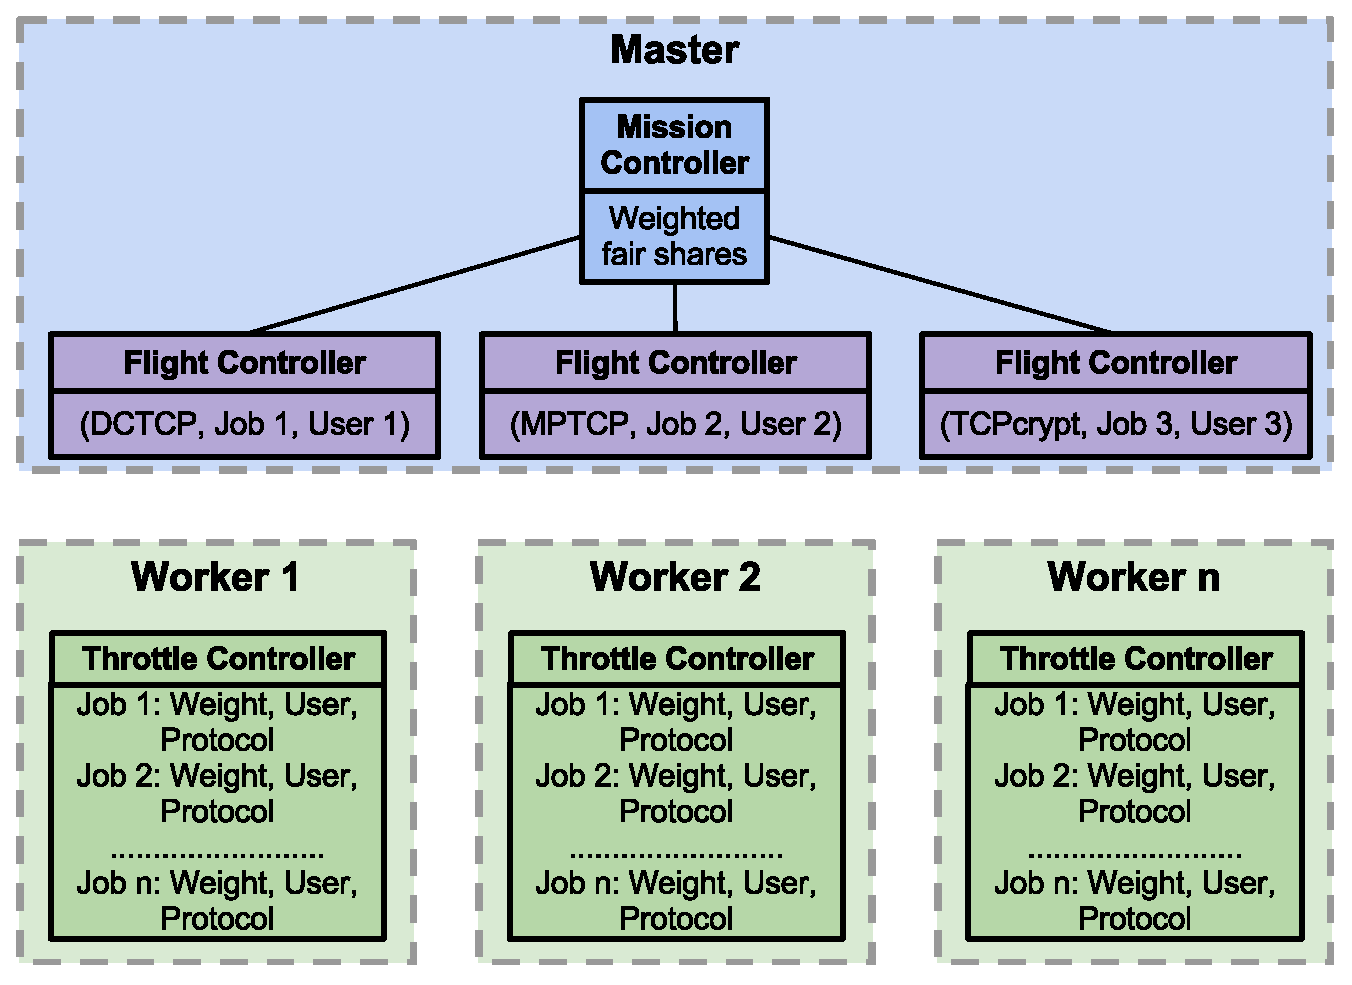
\includegraphics[width=0.8\textwidth]{MissionControl.eps}
    \caption{Mission Control architecture}
    \label{chap:design:fig:missioncontrol}
\end{figure}

\subsection{Mission Controller}
CIEL is capable of running multiple jobs at the same time. Mission Controller
resides alongside the CIEL master and coordinates transfer scheduling across
these jobs. To this end, it uses \emph{weighted fair sharing} to assign each
transfer a weight. In practice, this allows the sharing of each link in the
network proportional to these weights. In addition, weighted fair sharing
subsumes several policies including FIFO and priority~\cite{Chowdhury:2011:MDT}.
The values of these weights are subject to organizational goals and can be
calibrated on the basis of user profiles or job characteristics. For example,
jobs launched by \emph{Alice} can be given twice the priority of those launched
by \emph{Bob}. In the same vein, low latency jobs can be given higher priority
than batch-processing jobs. Similarly, to enable FIFO, weights can be assigned
proportional to job arrival time. By default we use performance-centric network
allocation to maximize parallelism~\cite{Kumar:2012:ACF}. For shuffle transfers
allocation is made on the basis of the number of target machines while per-flow
allocation is used for broadcast transfers. Concretely,

\begin{equation}
  share_{shuffle} = N
\end{equation}

\begin{equation}
  share_{broadcast} = N^2
\end{equation}

Where $N$ is the number of machines that the job uses. To distinguish between
shuffle and broadcast transfers, Mission Controller walks the task graph to
observe the relationships between tasks and their inputs and outputs (described
in the implementation section). In addition, transport protocols are selected on
the basis of job characteristics and the environment. For example, multi-path
TCP is selected if the host has more than one interface. Moreover, users can
explicitly specify a transport protocol at job submission time. In summary,
Mission Controller maintains cluster-wide state of resources and selects the
transport layer protocol for a particular transfer.

\subsection{Flight Controller}
Each transfer is associated with a Flight Controller that handles transport
specific resources. To this end, each FC implements the control plane of a
particular transport protocol and its various parameters.
For example, the multi-path TCP FC selects the number of flows per TCP
connection. Each FC is registered with the Mission Controller and receives its
weight assignment. It is important to highlight that to change the transport
protocol at runtime, the Mission Controller unregisters the existing FC for a
transfer and replaces it with a corresponding FC for the new protocol.

\subsection{Throttle Controller}
Unlike the Mission Controller and Flight Controller(s), which reside on the
master node, Throttle Controllers are present at every worker. Each TC receives
its transfer schedule from the FC and uses that information to handle all flows
on the worker. Each TC receives information for each FC (or job) for which it
has to schedule a transfer (or task). As a result, Throttle Controllers have to
maintain both scheduling and transport parameter state for each local flow.
Figure~\ref{chap:design:fig:missioncontrol} illustrates the architecture of
Mission Control.

\section{Implementation}
In this section, we present how Mission Control extends the implementation of
CIEL to enable multiple transports and transfer scheduling. We first discuss the
implementation features of CIEL which are important for Mission Control.

\subsection{CIEL Implementation}
CIEL represents the state of each job in a \emph{dynamic task graph} which
records the relation between tasks and objects in the form of a bipartite
graph~\cite{Murray:2011:CUE,Murray:2011:ADE}. The former is stored in a task
table while the latter is stored in an object table. The task table stores the
code and data dependencies of each task keyed by task ID. Similarly, the object
table stores the input and output objects for each task keyed by object ID. All
of this information is stored in the form of \emph{references}. CIEL enables a
number of references which are described in
Table~\ref{chap:implem:sec:ciel:tab:ref}. The master stores a table of dynamic
task graphs with one entry for each job in the job pool. In addition, worker
state is stored in a worker table.

\begin{table}
  \centering
  \begin{tabular}{| l || l |}
    \hline
	\textbf{Reference} & \textbf{Description} \\ \hline \hline
    Future & Represents an object that has not been created yet \\ \hline
    Concrete &  For objects that have concrete values and locations \\ \hline
    Value & Stores the actual values of small objects \\ \hline
    Error & Stores the error code of failed tasks \\ \hline
    Streaming & Enables streaming data between tasks \\ \hline
    Sweetheart & Represents loop-invariant data \\ \hline
    Tombstone & Represents objects that are no longer available due to worker
    failure
    \\ \hline
    Fixed & Enables a task to be fixed to a worker\\
    \hline
  \end{tabular}
  \caption{CIEL References}
  \label{chap:implem:sec:ciel:tab:ref}
\end{table}

Tasks are scheduled on workers from the worker table once their dependencies, in
the form of future references, become concrete references. The task table is
updated each time a new task is spawned. Moreover, objects are stored within an
\emph{object store} at each worker. All of this information is leveraged by
Mission Control to optimize data transfer (described below). This data-dependent
abstraction can be used to implement any distributed data flow. For instance, a
fixed two-stage MapReduce flow can be enabled by adding one output Reference
from each Map task as a dependency to each Reduce task. 

\newpage

\lstset{language=Java,
basicstyle=\ttfamily,
keywordstyle=\color{javapurple}\bfseries,
stringstyle=\color{javared},
commentstyle=\color{javagreen},
morecomment=[s][\color{javadocblue}]{/**}{*/},
numbers=left,
numberstyle=\tiny\color{black},
stepnumber=1,
captionpos=b,
numbersep=10pt,
tabsize=4,
showspaces=false,
showstringspaces=false}
\begin{lstlisting}[caption={\texttt{FirstClassJavaTask}
Interface},label={lst:firstclassjavatask}] 
public interface FirstClassJavaTask extends Serializable 
{   
   /* 
    * Enables the task to setup any local state
    */
	void setup();
	
   /*
    * Holds the actual code for execution
    */	
	void invoke() throws Exception;	
	
   /*
    * Returns an array of the dependencies of the task
    */
	Reference[] getDependencies();
}
\end{lstlisting}

As mentioned earlier, tasks are scheduled once their dependencies become
concrete. To facilitate this, each \emph{concrete reference} consists of a name,
location and size. Objects are retrieved by sending an HTTP GET request with the
name of the object to the location\footnote{In case the reference has multiple
locations, the request is directed on the basis of network locality or at
random.} specified in the concrete reference. Under the hood,
PycURL\footnote{\url{http://pycurl.sourceforge.net/}}, a Python interface to
libcURL\footnote{\url{http://curl.haxx.se/libcurl/}} is used to fetch the
object. libcURL is a URL transfer library that supports multiple protocols
including HTTP and FTP. Furthermore, CIEL also allows partially written objects
to be pipelined between tasks through \emph{stream references}. Finally, CIEL
exposes a language-agnostic interface that can be used to spawn tasks in any
programming language, including Skywriting, Python, Java, and C. This
\emph{first-class executor} enables a running task to, (1) Spawn other tasks,
(2) Delegate its output(s), and (3) Create new objects on the fly.
In this thesis, we focus on the Java first-class executor, but the design is
applicable to executors in any language.

\subsubsection{Java First-class Executor}
Tasks in Java can be written by implementing the \texttt{FirstClassJavaTask}
interface shown in Listing~\ref{lst:firstclassjavatask}. In addition, the
platform also provides a \texttt{ConstantNumOutputsTask} interface which extends
\texttt{FirstClassJavaTask} with a \texttt{getNumOutputs} method to hold the
number of outputs of a task. Finally, tasks also have access to a \texttt{Ciel}
object which exposes a number of helper methods, some of which are described in
Table~\ref{chap:implem:sec:ciel:tab:task}.

\begin{table}
  \centering
  \begin{tabularx}{6in}{|X|X|} 
    \hline
	\textbf{Method} & \textbf{Description} \\ \hline \hline
    \texttt{Ciel.args} & Returns user-supplied arguments \\ \hline
    \texttt{Ciel.spawn} & Spawns a task with the given code dependency \\ \hline
    \texttt{Ciel.tailSpawn} & Spawns a task with the given code dependency and
    delegates the expected output(s) of the current task to it
    \\ \hline
    \texttt{Ciel.RPC.getStreamForReference} & Opens the object defined
    in the reference in pipelining mode \\ \hline
    \texttt{Ciel.RPC.getFilenameForReference} & Fetches the object defined in
    the reference \\ \hline
     \texttt{Ciel.RPC.getOutputFilename} & Creates a new reference to hold the
     output(s) of the task \\ \hline
 \end{tabularx} 
  \caption{Important CIEL First-class Java Executor helper methods}
  \label{chap:implem:sec:ciel:tab:task}
\end{table}

\subsection{Mission Control Implementation}

\begin{table}
  \centering
  \begin{tabularx}{5in}{|X|X|} 
    \hline
	\textbf{Policy} & \textbf{Description} \\ \hline \hline
    FIFO & Jobs are assigned weights on the basis of their arrival time. \\
    \hline 
    Priority & Job priorities are specified by the user. A job with a priority
    of 2 is assigned a weight which is double the weight assigned to a
    priority 1 job.\\ \hline 
    Fair & Jobs are assigned equal weights.\\ \hline 
    Performance-centric & Weights are assigned to maximize performance
    parallelism. A broadcast transfer is assigned twice the weight of a shuffle
    transfer.\\
    \hline
 \end{tabularx} 
  \caption{List of weight assignment policies supported by Mission Control}
  \label{chap:implem:sec:ciel:tab:policies}
\end{table}

Mission Control extends both the Python implementation of CIEL and its
first-class Java executor. The
former\footnote{\url{https://github.com/ZubairNabi/ciel}} is modified to
implement Mission Controller, Flight Controller, and Throttle Controller while
the latter\footnote{\url{https://github.com/ZubairNabi/ciel-java}} is extended
to enable concurrent data fetch threads. In addition, a number of Bash
scripts\footnote{\url{https://github.com/ZubairNabi/ciel/tree/master/scripts}}
have also been written to manage CIEL and the working environment. We first
describe the changes to the master followed by changes to the worker.

\subsubsection{Master}\label{chap:implem:sec:ciel:subsec:master}
At the master, the Mission Control implementation consists of two classes to
represent Mission Controller and Flight Controller, respectively. We modified
the CIEL representation of a job to associate each job with a weight and a
Flight Controller. The Mission Controller thread is spawned during the
initialization of the master. It maintains an updated list of currently running
jobs along with their tasks and dependencies. In addition, it is also associated
with a policy which dictates per-job weight assignment. The list of currently
supported policies is given in Table~\ref{chap:implem:sec:ciel:tab:policies}.
The weights assigned by these policies determine the number of concurrent flows
that each job can initiate during a data fetch. These weights are updated every
second depending on the selected policy.
Table~\ref{chap:implem:sec:ciel:tab:policiesassign} shows how weights are
assigned under different policies for 2 jobs: Job 1 and Job 2. The maximum
number of concurrent flows per host is 10 and Job 1 arrives first and is
assigned all 10 flows.

\begin{table}
  \centering
  \begin{tabularx}{5in}{|X|X|} 
    \hline
	\textbf{Policy} & \textbf{Weights} \\ \hline \hline
    FIFO & As soon as Job 2
    arrives, it is assigned a weight of 3 and the weight of Job 1 is decreased
    to 7. \\ \hline 
    Priority & Job 2 arrives and has a higher priority than Job 1. Job 2 is
    assigned a weight of 7 and the weight of Job 1 is decreased to 3. \\
    \hline 
    Fair & Job 2 arrives and is assigned a weight of 5 and the weight of Job
    1 is decreased to 5.\\ \hline 
    Performance-centric & Job 1 has a shuffle transfer while Job 2 has a
    broadcast transfer. Job 2 arrives and is assigned a weight of 7 and the
    weight of Job 1 is decreased to 3.\\
    \hline
 \end{tabularx} 
  \caption{Illustrative example of weight assignment under different policies
  for 2 jobs}
  \label{chap:implem:sec:ciel:tab:policiesassign}
\end{table}

Be default, Mission Controller uses the
performance-centric~\cite{Kumar:2012:ACF} policy in which weights are assigned
on the basis of application semantics. To this end, Mission Controller performs
a breadth-first search of the dynamic task graph for each job. If the tasks in a
stage have one reference from each task in the previous stage as a dependency,
the stage is marked as a shuffle. In contrast, if all of the output references
of the previous stage are dependencies of tasks in the subsequent stage, then
the stage is marked as a broadcast. This information is then used to assign
twice the weight of a shuffle transfer to a broadcast transfer. In addition, the
current implementation supports four transport protocols. These protocols and
their selection criteria is given in
Table~\ref{chap:implem:sec:ciel:tab:protocols}. It is important to highlight
that any transport protocol can easily be added to Mission Controller by
extending the Flight Controller class.

\begin{table}
  \centering
  \begin{tabularx}{5in}{|X|X|} 
    \hline
	\textbf{Protocol} & \textbf{Description} \\ \hline \hline
    TCP & The default transport. \\ \hline
    MPTCP & Selected when the host has more than one interface. In case MPTCP is
    selected, the number of concurrent data fetch connections per host are
    turned into concurrent sub-flows under the same MPTCP connection.
    \\ \hline 
    DCTCP & Selected when the switches in the network support ECN.
    \\ \hline
    TCPcrypt & Not selected by the framework. It needs to be explicitly enabled
    during job submission time by the user.
    \\
    \hline
 \end{tabularx} 
  \caption{List of transport protocols supported by Mission Control}
  \label{chap:implem:sec:ciel:tab:protocols}
\end{table}

To implement the communication model of Mission Control, we use the Isis2
virtual synchrony library.
Isis2~\cite{Birman:2012:OCW}\footnote{\url{http://isis2.codeplex.com/}} is a
toolkit which implements the virtual synchrony model and simplifies the design
of distributed applications. It provides a number of reliable multicast
primitives with varying ordering guarantees. Durability is ensured through a
mechanism dubbed, \emph{amnesia freedom}, that delays the application till an
acknowledgement has been received from every replica. This mechanism is exposed
through a barrier primitive called \emph{Flush}, that delays till all prior
multicast messages have reached their destinations. Isis2 also provides a number
of send primitives including a FIFO-ordered send as well as a \emph{SafeSend},
which implements a virtually synchronous version of
Paxos~\cite{Lamport:1998:PP}. Isis2 targets C\# development but can be used
within IronPython\footnote{\url{http://ironpython.net/}}. Therefore, to make use
of Isis2 we first port CIEL to IronPython. In our implementation, CIEL workers
are organized into a virtual group. The Mission Controller multicasts weight
allocations and transport semantics to the virtual group using the Isis2 send
primitive. This enables all workers to have the same consistent view of the
transport semantics. Isis2 uses a ``dynamically reconfigurable services'' model
as a consensus mechanism known as the ORACLE. We currently run the ORACLE
service at the master node but for large-scale deployments it would be more
feasible to have more than one ORACLE.

\subsubsection{Worker}\label{chap:implem:sec:ciel:subsec:workers}
\sloppy At the worker, the implementation consists of a Throttle Controller
instance that receives data transfer semantics from the Mission Controller. In
particular, it distributes its total number of flows among the executing tasks.
This number is bounded by \texttt{pycurl.M\_MAXCONNECTS} at every host.
In CIEL, executors in different programming languages communicate with the
underlying framework using JavaScript Object Notation
(JSON)\footnote{\url{http://www.json.org/}} based RPC. For instance, the methods
in Table~\ref{chap:implem:sec:ciel:tab:task} are implemented through this
interface. To enable the Throttle Controller to allocate concurrent flows to
each executing task, the RPC methods are extended to include a
\texttt{Ciel.RPC.getConcurrentFilenamesForReferences} method to spawn multiple
threads to make concurrent calls to the built-in
\texttt{Ciel.RPC.getFilenameForReference} method. The number of these threads
per task is equal to its concurrent flow quota. As a result, the Throttle
Controller is able to distribute its \texttt{pycurl.M\_MAXCONNECTS} number of
concurrent flows among the executing tasks. Moreover, on instructions from the
Mission Controller, the Throttle Controller switches between transport protocols
using the Linux \texttt{sysctl}\footnote{\texttt{sysctl} enables the
modification of kernel parameters at runtime.} interface.
 
\chapter{Evaluation}\label{chapter:evaluation}
This section presents a thorough evaluation of Mission Control. We first
describe the testbed.

\section{Testbed}
For all our experiments we use an AMD Opteron 6168 with 48 x86\_64 cores, with
each core clocked at 2 GHz with a 512 KB cache. The system has 64 GB of DDR3
RAM, 1 TB of HDD, and 1 Gbps network connectivity. In addition, the system is
also provisioned with a 256 GB solid state drive\footnote{We use the SSD to
negate the effect of disk I/O on shuffle time.}.

On the software side, the system runs a Debian-based Linux kernel version
3.2.x.x. We use Linux Containers
(LXC)\footnote{\url{http://lxc.sourceforge.net/}} for lightweight
virtualization. 41 containers were created to host the
CIEL\footnote{\url{https://github.com/mrry/ciel}} master and workers. The
container housing the CIEL master was pinned to 4 CPU cores while the rest of
the 40 containers, running CIEL workers, were pinned to 1 CPU core each. In
addition, the former was provisioned with 100 GB of HDD space in the form of a
logical volume while the latter were provisioned with 20 GB of the same each.
The SSD is shared by all. Finally,
OpenVSwitch~\cite{Pfaff:2009:ENI}\footnote{\url{http://openvswitch.org/download/}}
is used as the L2 fabric with 1 Gbps link speed.

For all our experiments, we use a custom MapReduce Java library written for
CIEL\footnote{\url{https://github.com/ZubairNabi/ciel-java/tree/master/examples/src/main/java/com/asgow/ciel/examples/mapreduce}}.
This enables us to (a) Easily port Hadoop applications to CIEL, (b) Monitor and
log phase-wise task execution. We implement different topologies by connecting
and rate-limiting OpenVSwitch-enabled bridges. To monitor the CPU and network
usage of each worker, we poll the \texttt{/proc} filesystem. Unless otherwise
stated, all application data (input, intermediate, and output) is stored on the
SSD. In addition, all error bars represent the standard deviation.

\section{Analysis of network behaviour of CIEL on different workloads}
To gain some insight into the network behaviour of CIEL, we first conduct a
series of experiments using an I/O-intensive and a CPU-intensive application.
For the former we use sort and for the latter we use \emph{k}-means clustering.

\subsection{Sort}
In our sort implementation, the map and reduce functions are identity while the
underlying framework itself performs the actual sort. In this experiment, our
goal is to study the effect of data size on the shuffle and the overall job
completion time. A 20 GB text dataset was synthetically generated to ensure
equal partitioning and equal distribution of keys, i.e. task times are not
biased by unequal work distribution. Each file in the dataset is 64 GB in size,
with 640 files in total. Each file is given as input to a single map task while
the number of reduce tasks is kept constant at 40\footnote{One per CIEL
worker.}. Each CIEL worker is configured for a single task slot. In this setup,
all 41 containers are connected to the same switch.

\begin{figure}[h!]
  \centering
    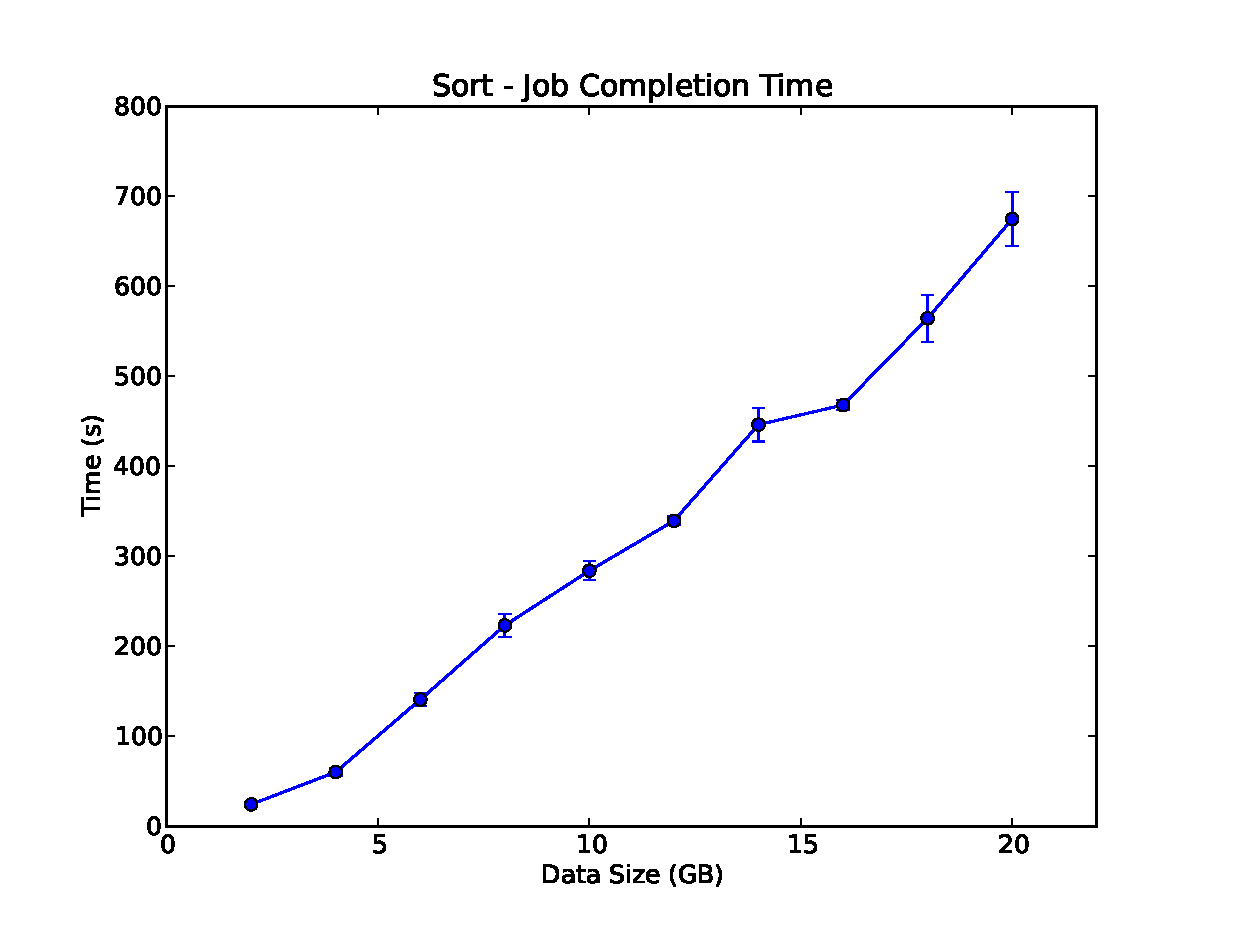
\includegraphics[width=0.8\textwidth]{sort.eps}
    \caption{Sort - Job Completion Time}
    \label{chap:eval:sec:ciel:fig:sort}
\end{figure}

\begin{figure}[h!]
  \centering
    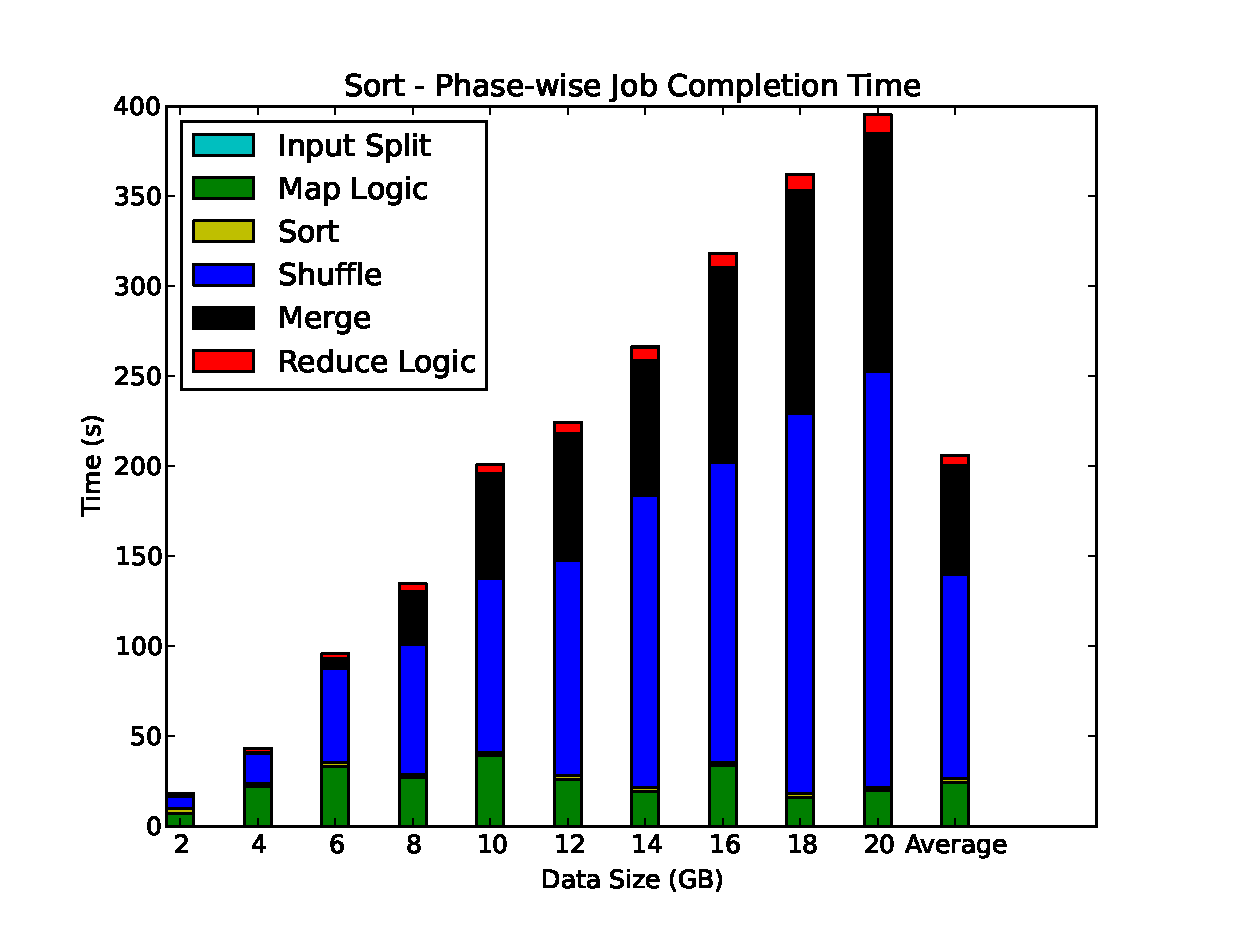
\includegraphics[width=0.8\textwidth]{sort_phase.eps}
    \caption{Sort - Phase-wise Job Completion Time}
    \label{chap:eval:sec:ciel:fig:sortphase}
\end{figure}

Figure~\ref{chap:eval:sec:ciel:fig:sort} shows the results of 10 runs of sort
for input data size varied from 2 GB to 20 GB. The job completion time linearly
increases with the increase in input. A phase-wide breakdown of the job
completion time in Figure~\ref{chap:eval:sec:ciel:fig:sortphase} reveals that
the shuffle phase accounts for up to half of the total time.

To understand the effect of the application on system resources, we plot the CPU
and network usage of sort for input data of size 2, 10, and 20 GB in
Figure~\ref{chap:eval:sec:ciel:fig:sortres}. We see that there is a spike in
network traffic during the shuffle phase while otherwise the network is
under-utilized.

\begin{figure}[h!]
        \begin{subfigure}[b]{0.33\textwidth}
                \centering
                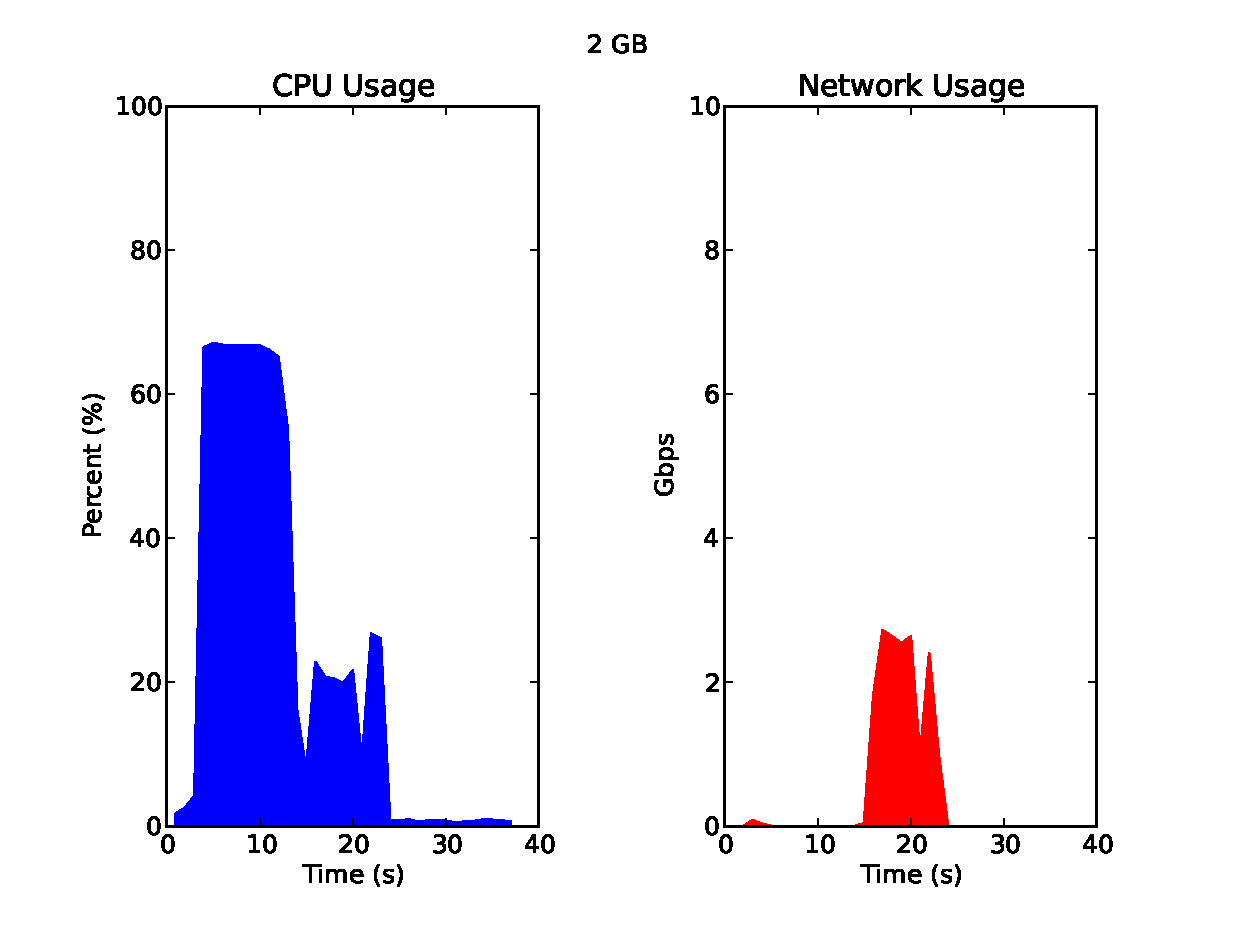
\includegraphics[width=\textwidth]{32maps.csv.eps}
                \caption{2 GB - 32 maps}
                \label{fig:2GBsortres}
        \end{subfigure}%
        \begin{subfigure}[b]{0.33\textwidth}
                \centering
                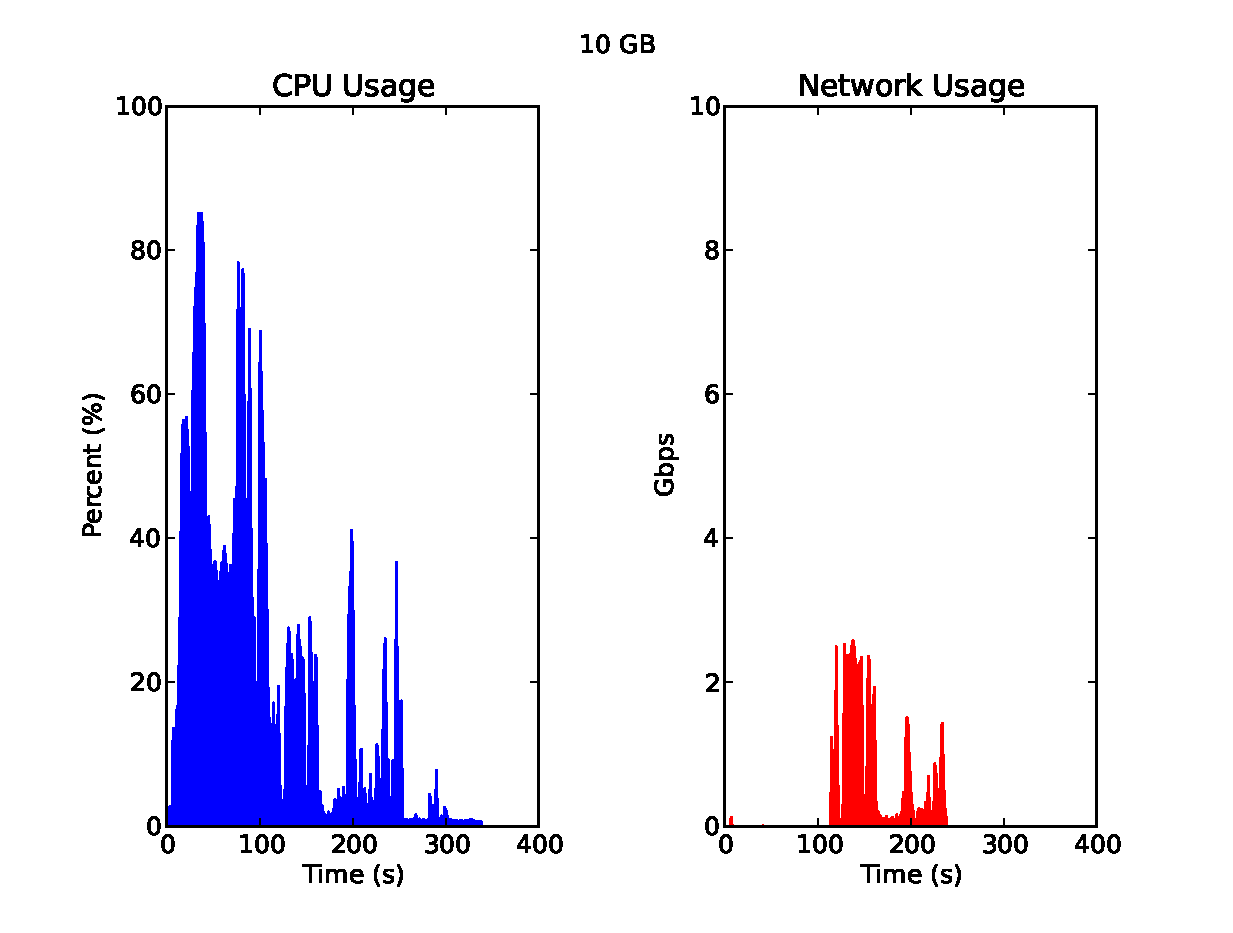
\includegraphics[width=\textwidth]{160maps.csv.eps}
                \caption{10 GB - 160 maps}
                \label{fig:10GBsortres}
        \end{subfigure}
        \begin{subfigure}[b]{0.33\textwidth}
                \centering
                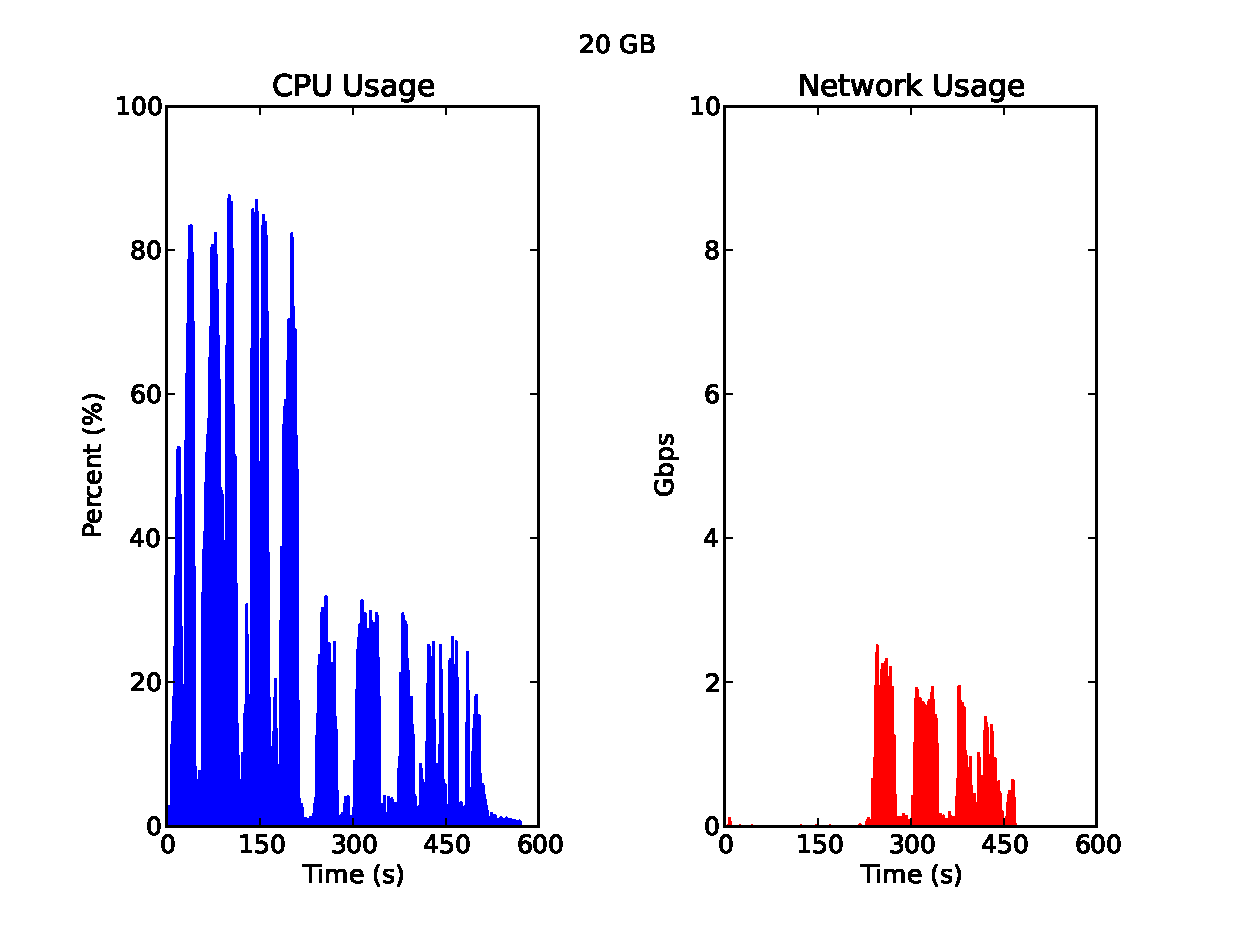
\includegraphics[width=\textwidth]{320maps.csv.eps}
                \caption{20 GB - 320 maps}
                \label{fig:20GBsortres}
        \end{subfigure}
        \caption{CPU and Network usage of sort}
        \label{chap:eval:sec:ciel:fig:sortres}
\end{figure}

\subsection{\emph{k}-means clustering}
We now consider \emph{k}-means clustering, a CPU intensive application. This
application takes advantage of CIEL's dynamic task generation by iterating till
the result is within an acceptable value. The CIEL port of this application is
identical to its Mahout\footnote{\url{http://mahout.apache.org/}} implementation
without requiring an external driver. The map function assigns each input point
to its nearest cluster based on a distance metric. The reduce function sums up
the values and checks if they have converged. In case they have not, it launches
the next iteration of the application. To evaluate this application, we
generated 64 MB cluster files with 80,000 dense vectors and \emph{k}, cluster
center, value of 100. Each vector contains 100 double-precision
values~\cite{Murray:2011:CUE}.

\begin{figure}[h!]
  \centering
    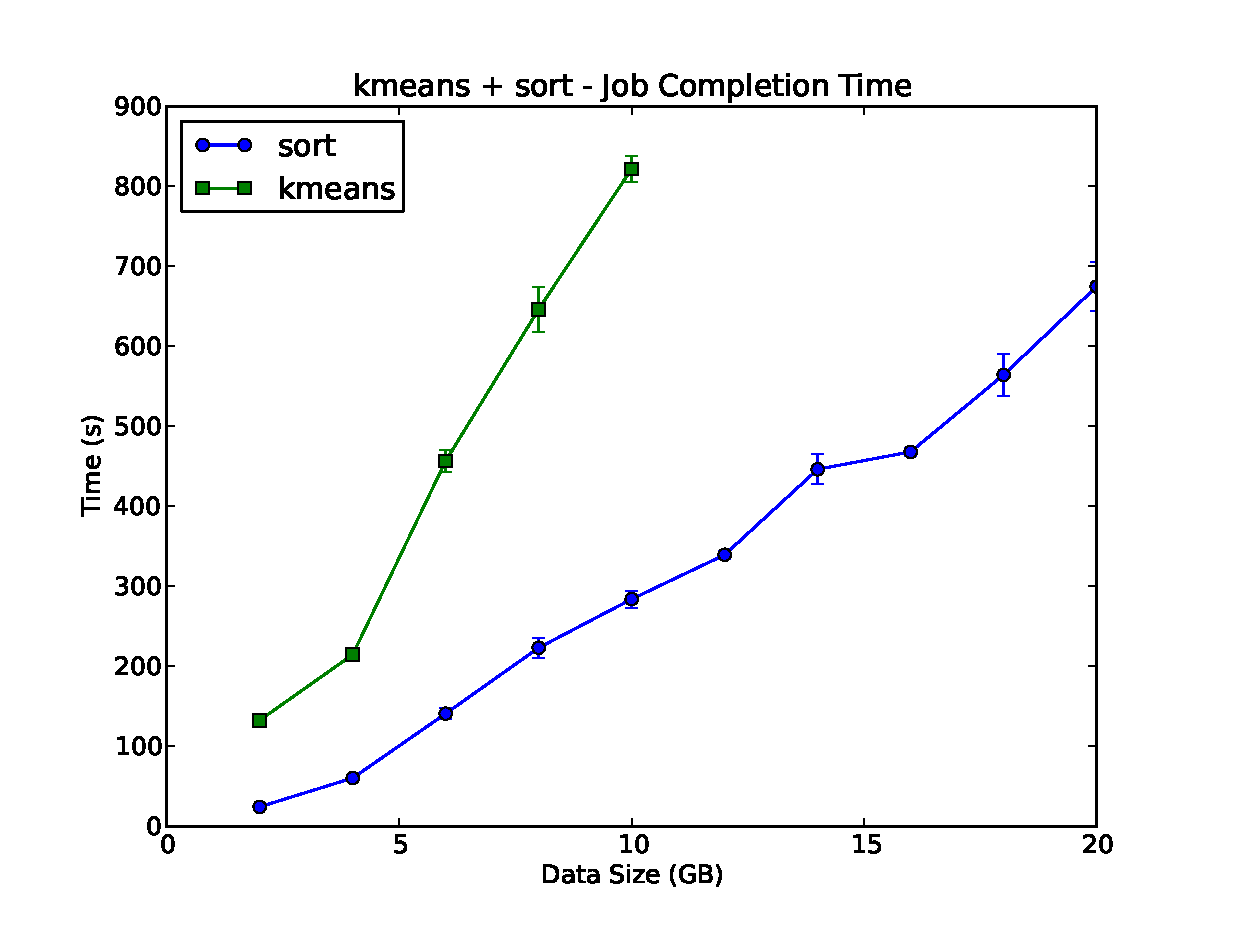
\includegraphics[width=0.8\textwidth]{kmeans_sort.eps}
    \caption{Sort and \emph{k}-means Job Completion Time}
    \label{chap:eval:sec:ciel:fig:kmeans}
\end{figure}

Figure~\ref{chap:eval:sec:ciel:fig:kmeans} plots the job completion time of
\emph{k}-means as a function of the input data size. In contrast to sort, the
execution time of \emph{k}-means shoots up with an increase in input. This is
due to the CPU intensive nature of the application as well as the dynamic task
generation. The CPU and network usage of the application is shown in
Figure~\ref{chap:eval:sec:ciel:fig:kmeansres}. Again in contrast to sort, we see
network and CPU activity throughout the course of the execution.

\begin{figure}[h!]
        \begin{subfigure}[b]{0.33\textwidth}
                \centering
                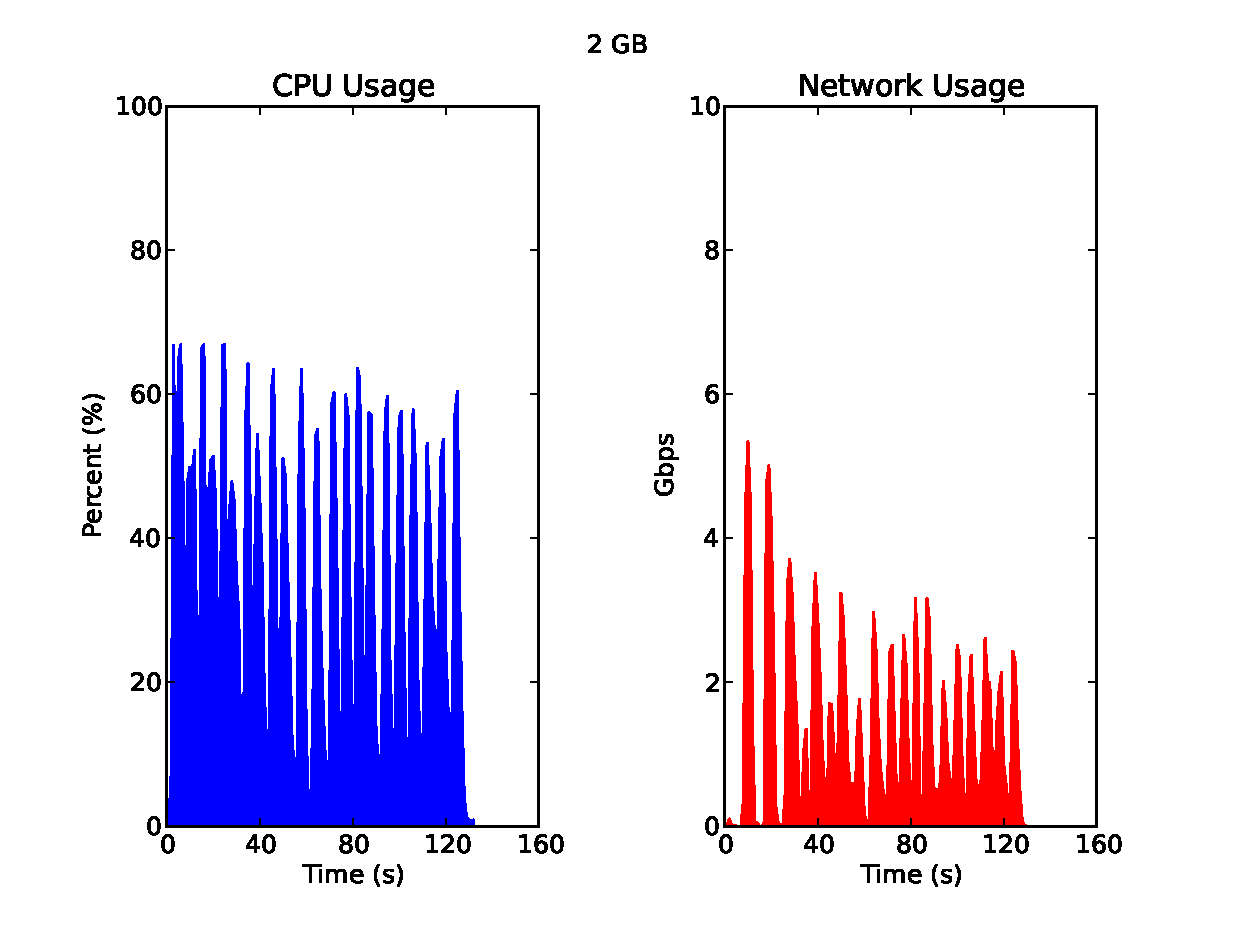
\includegraphics[width=\textwidth]{kmeans32.csv.eps}
                \caption{2 GB}
                \label{fig:2GBkmeansres}
        \end{subfigure}%
        \begin{subfigure}[b]{0.33\textwidth}
                \centering
                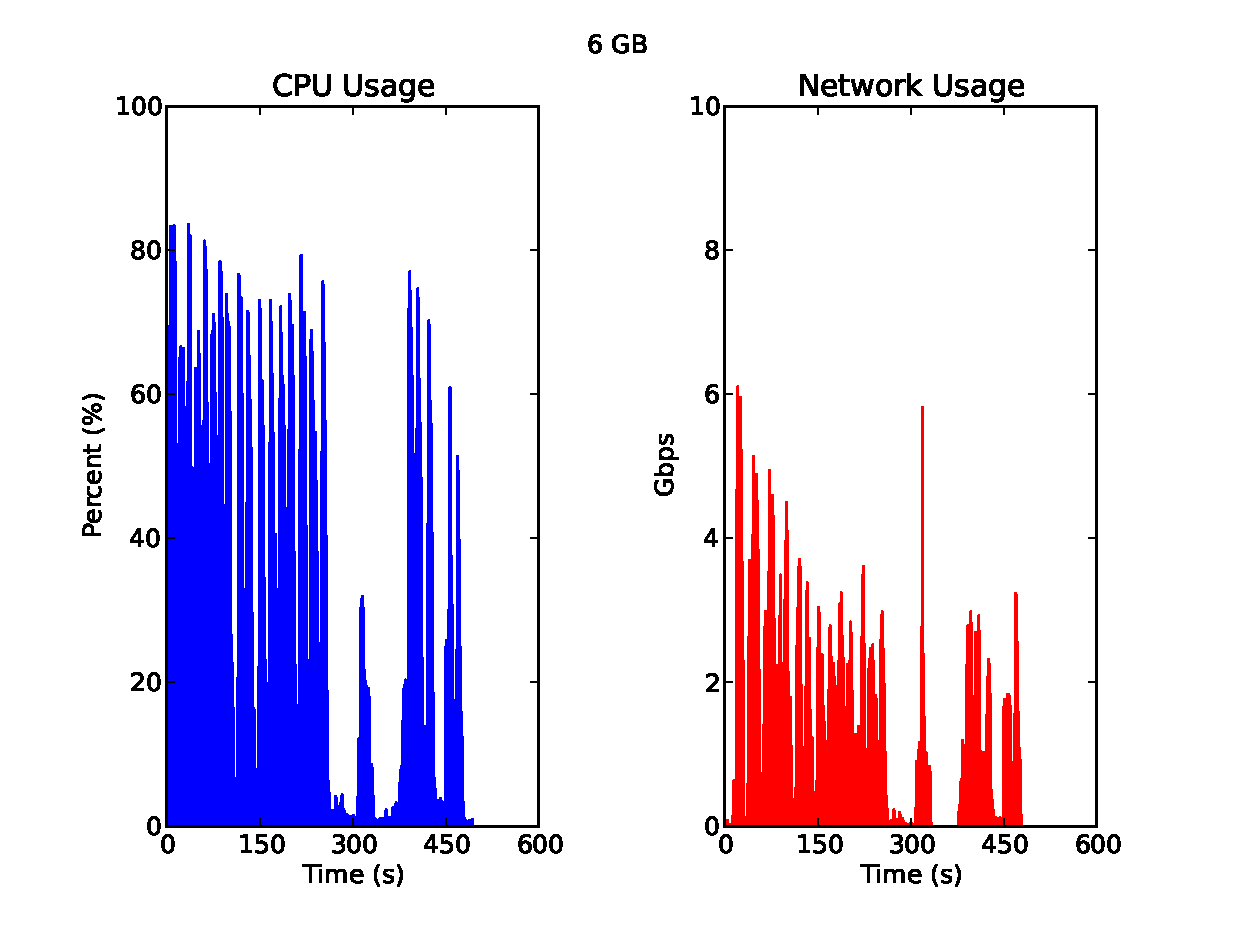
\includegraphics[width=\textwidth]{kmeans96.csv.eps}
                \caption{6 GB}
                \label{fig:6GBsortres}
        \end{subfigure}
        \begin{subfigure}[b]{0.33\textwidth}
                \centering
                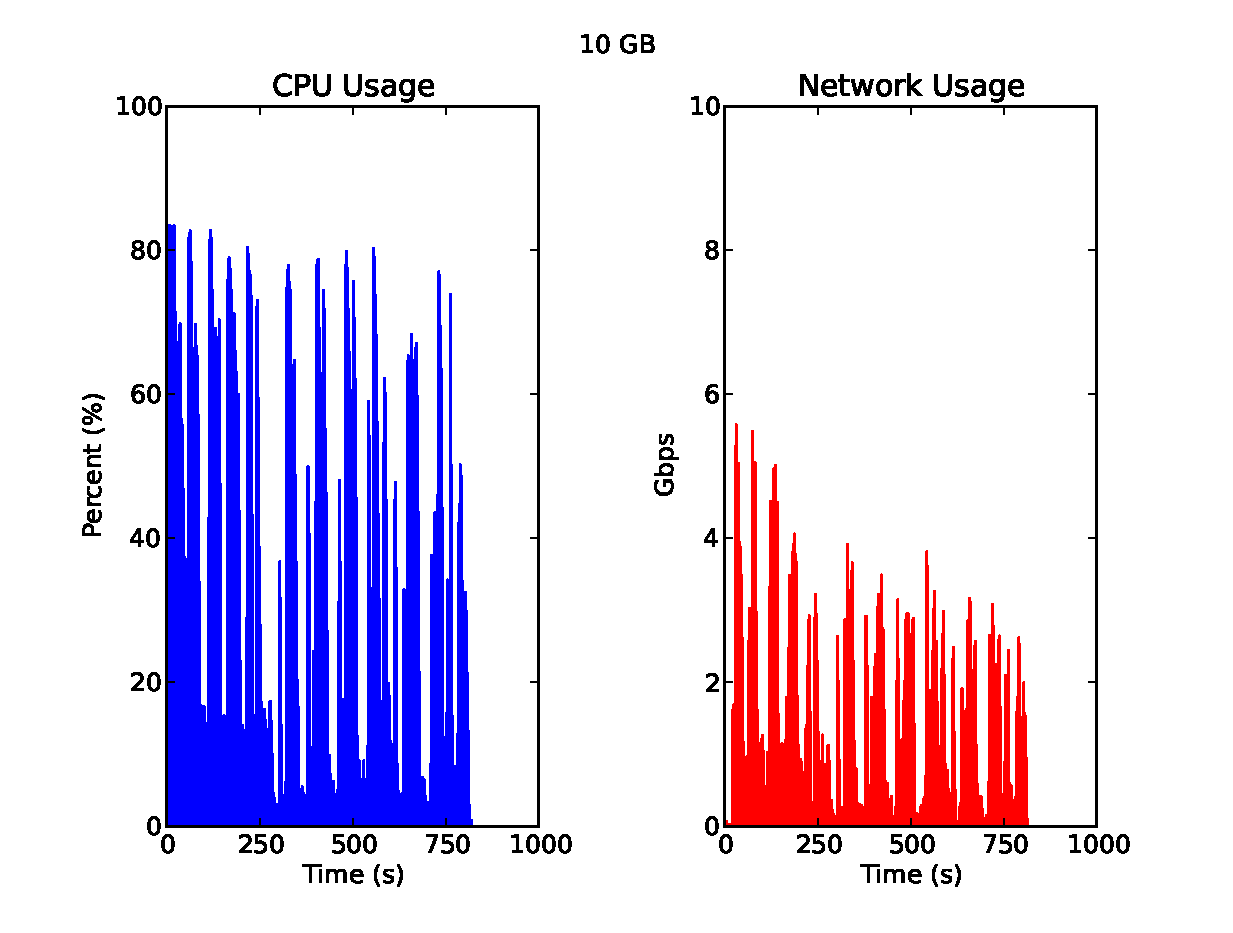
\includegraphics[width=\textwidth]{kmeans160.csv.eps}
                \caption{10 GB}
                \label{fig:10GBsortres}
        \end{subfigure}
        \caption{CPU and Network usage of \emph{k}-means}
        \label{chap:eval:sec:ciel:fig:kmeansres}
\end{figure}

\section{Performance of CIEL using different transport semantics}
 \begin{figure}[h!]
  \centering
    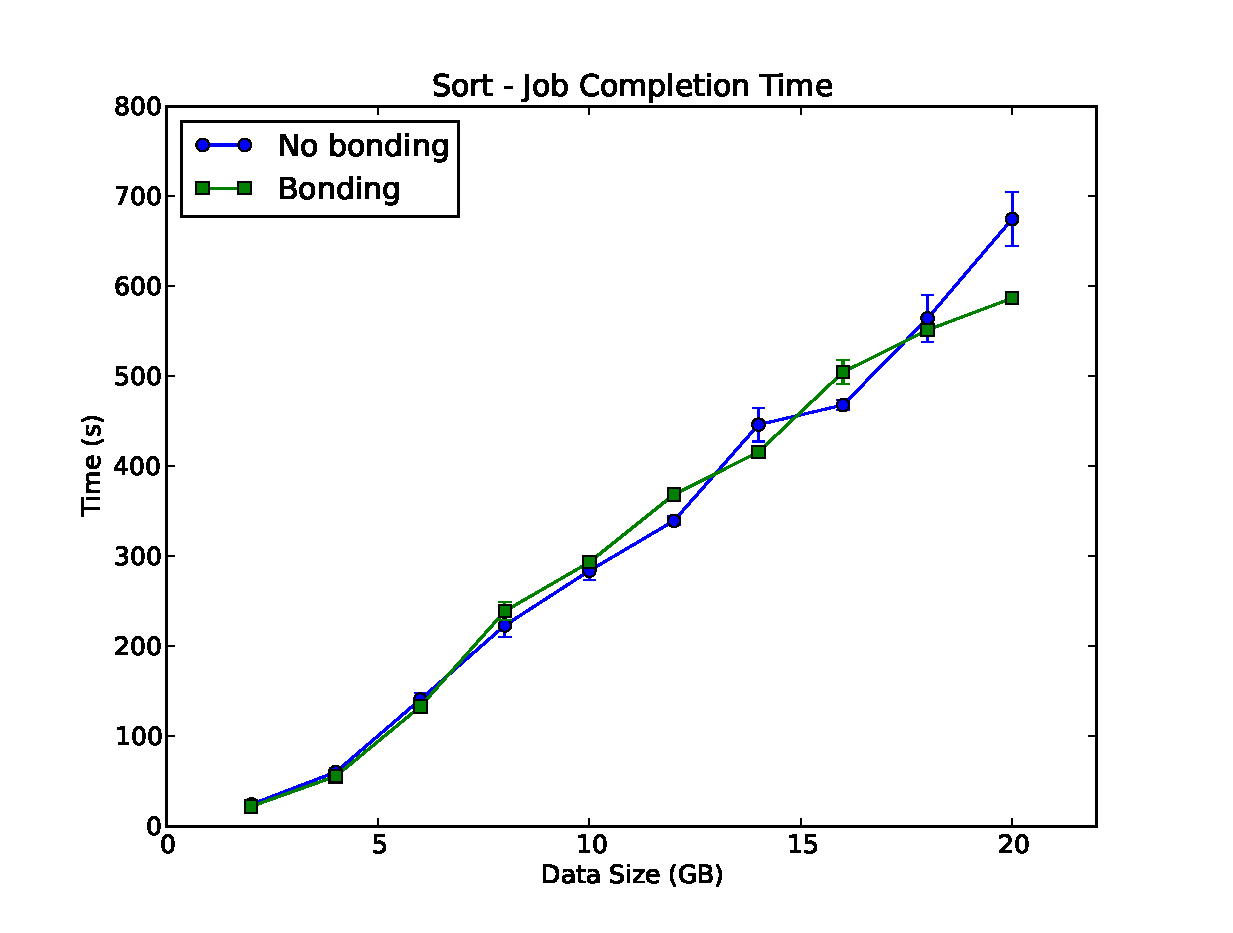
\includegraphics[width=0.8\textwidth]{sort_bonding.eps}
    \caption{Sort with Bonding - Job Completion Time - Star topology}
    \label{chap:eval:sec:ciel:fig:sortbonding}
\end{figure}

\begin{figure}[h!]
  \centering
    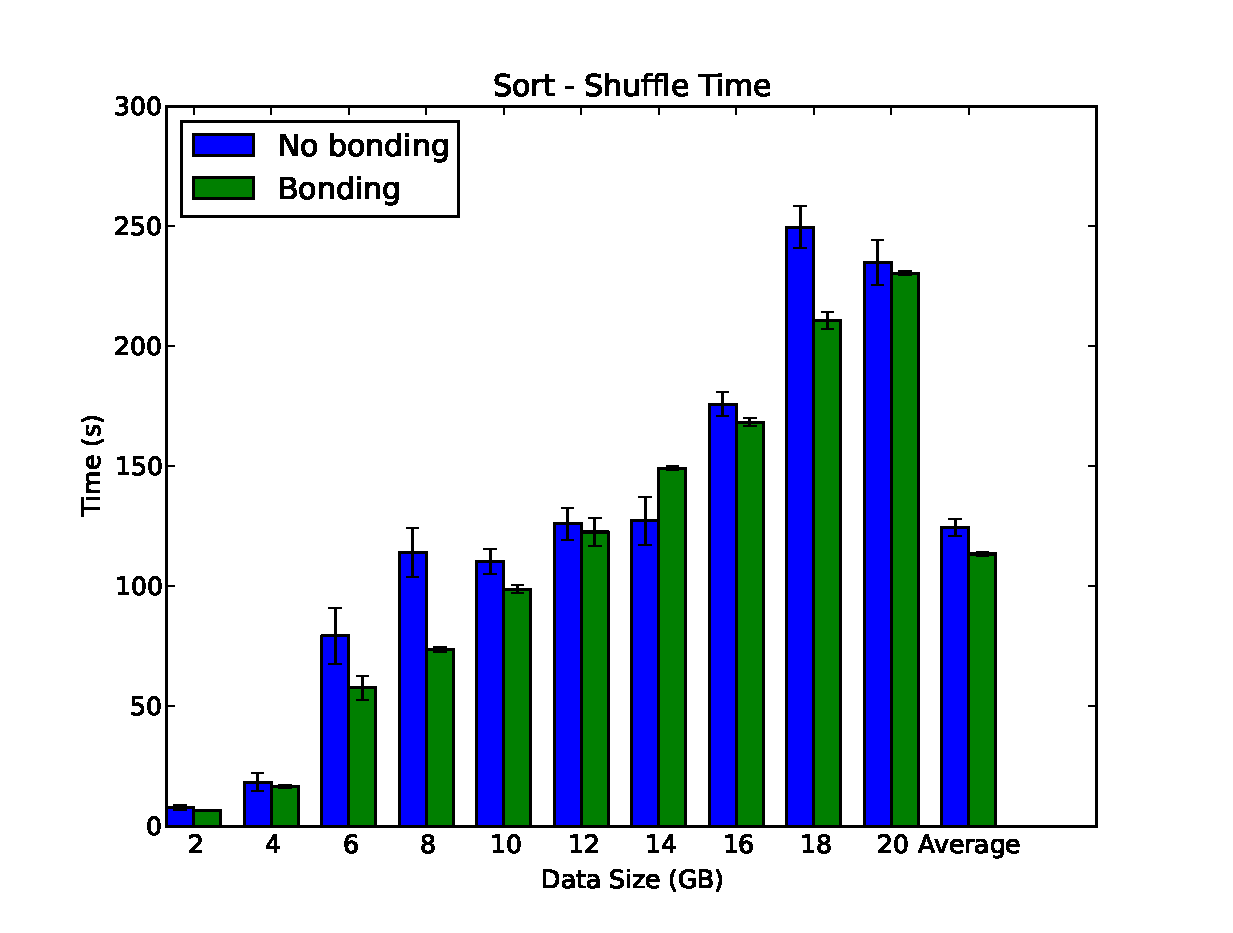
\includegraphics[width=0.8\textwidth]{shuffle_bonding_no_bonding.eps}
    \caption{Sort with Bonding - Shuffle Time - Star topology}
    \label{chap:eval:sec:ciel:fig:sortshuffle}
\end{figure}

In this section we evaluate the performance of CIEL under different transport
semantics.

\subsection{Ethernet Bonding}
We first evaluate Ethernet bonding. We add an extra interface to each container
and use the \texttt{bonding} module in Linux to bond both interfaces per
container. To stripe traffic from the same TCP connection over the interfaces,
we make use of the \texttt{balance-rr} bonding mode.
Figure~\ref{chap:eval:sec:ciel:fig:sortbonding} shows the job completion time of
CIEL sort with and without Ethernet bonding. Both methods exhibit the same
behaviour.

To gain more insight, in Figure~\ref{chap:eval:sec:ciel:fig:sortshuffle} we only
focus on the shuffle time. On average, Ethernet bonding improves shuffle time
by 9\%.

\subsection{Multiple Paths}
As mentioned earlier, emerging data center topologies aim to provide multiple
paths between each source and destination pair. In this experiment, we evaluate
whether multiple-path aware protocols can achieve higher throughput. We use
MPTCP\footnote{\url{http://mptcp.info.ucl.ac.be/}}~\cite{Raiciu:2012:HHC} as a
representative protocol. In this experiment we benchmark the performance of our
sort application using TCP, TCP with bonding, and MPTCP. Out setup consists of 9
containers: 1 master and 8 workers. We vary the input dataset size between 1 GB
and 4 GB\footnote{Due to a bug in the MPTCP kernel implementation we are unable
to scale out beyond 9 hosts.}.
Figure~\ref{chap:eval:sec:ciel:fig:sortshufflemptcp} plots the shuffle time for
TCP, TCP with bonding, and MPTCP. Surprisingly, MPTCP performs poorly in
comparison to standard TCP. We attribute this to 3 factors: (1) Additional
checksum for data sequence mapping (DSM)~\cite{Raiciu:2012:HHC}, (2) The use of
short-flows for which MPTCP achieves lower throughput~\cite{Raiciu:2010:DCN},
and (3) The immaturity of the MPTCP kernel implementation.
Figure~\ref{chap:eval:sec:ciel:fig:sortresmptcp} shows the CPU and network
utilization of TCP and MPTCP for a 4 GB dataset. MPTCP does not ramp up to
achieve the same throughput as TCP. We believe that these results do not
accurately reflect the true potential of MPTCP and evaluation on a different
set-up would yield more representative results.


 \begin{figure}[h!]
  \centering
    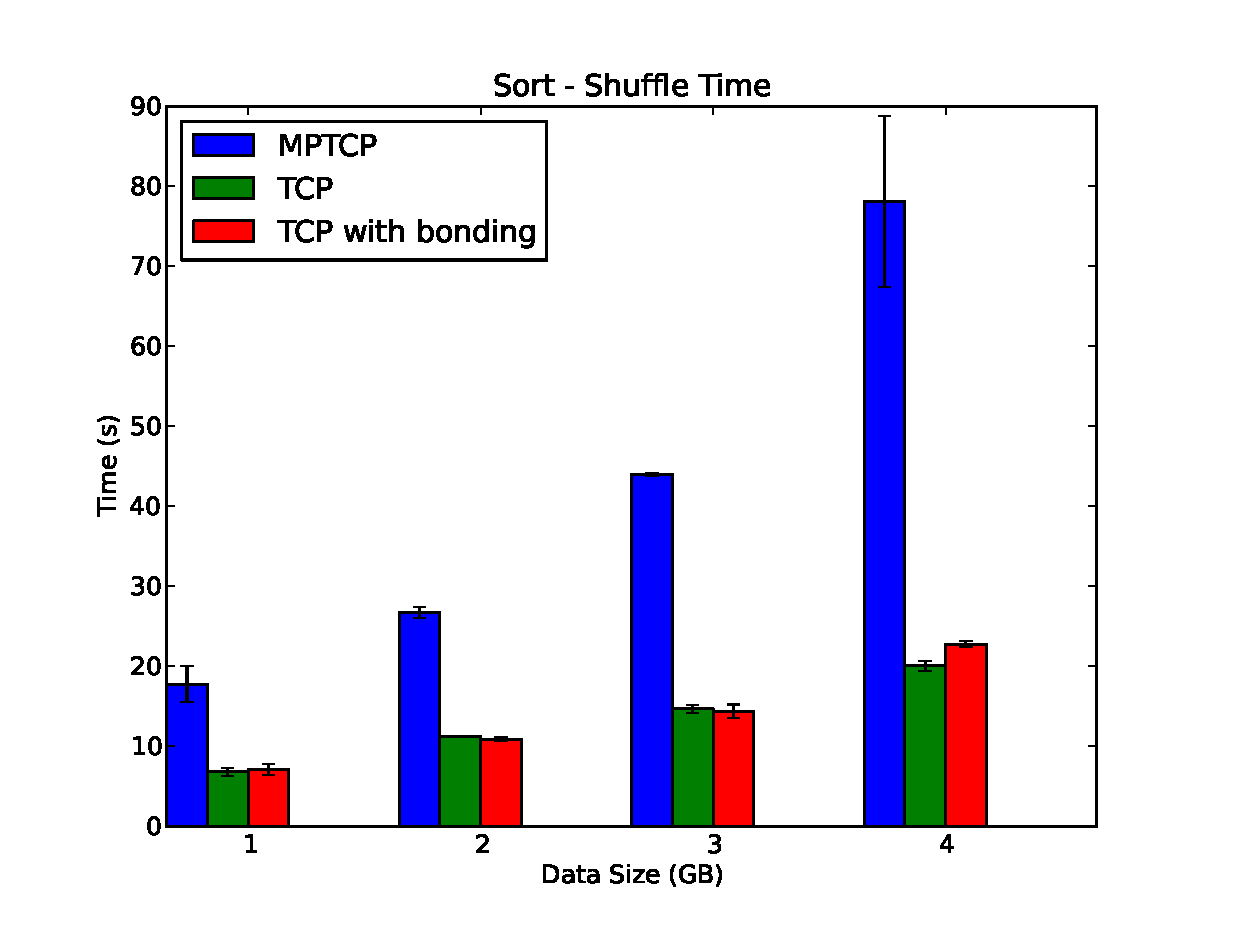
\includegraphics[width=0.8\textwidth]{shuffle_sort_mptcp.eps}
    \caption{Sort TCP vs. MPTCP - Shuffle Time - Star topology}
    \label{chap:eval:sec:ciel:fig:sortshufflemptcp}
\end{figure}

\begin{figure}[h!]
        \begin{subfigure}[b]{0.49\textwidth}
                \centering
                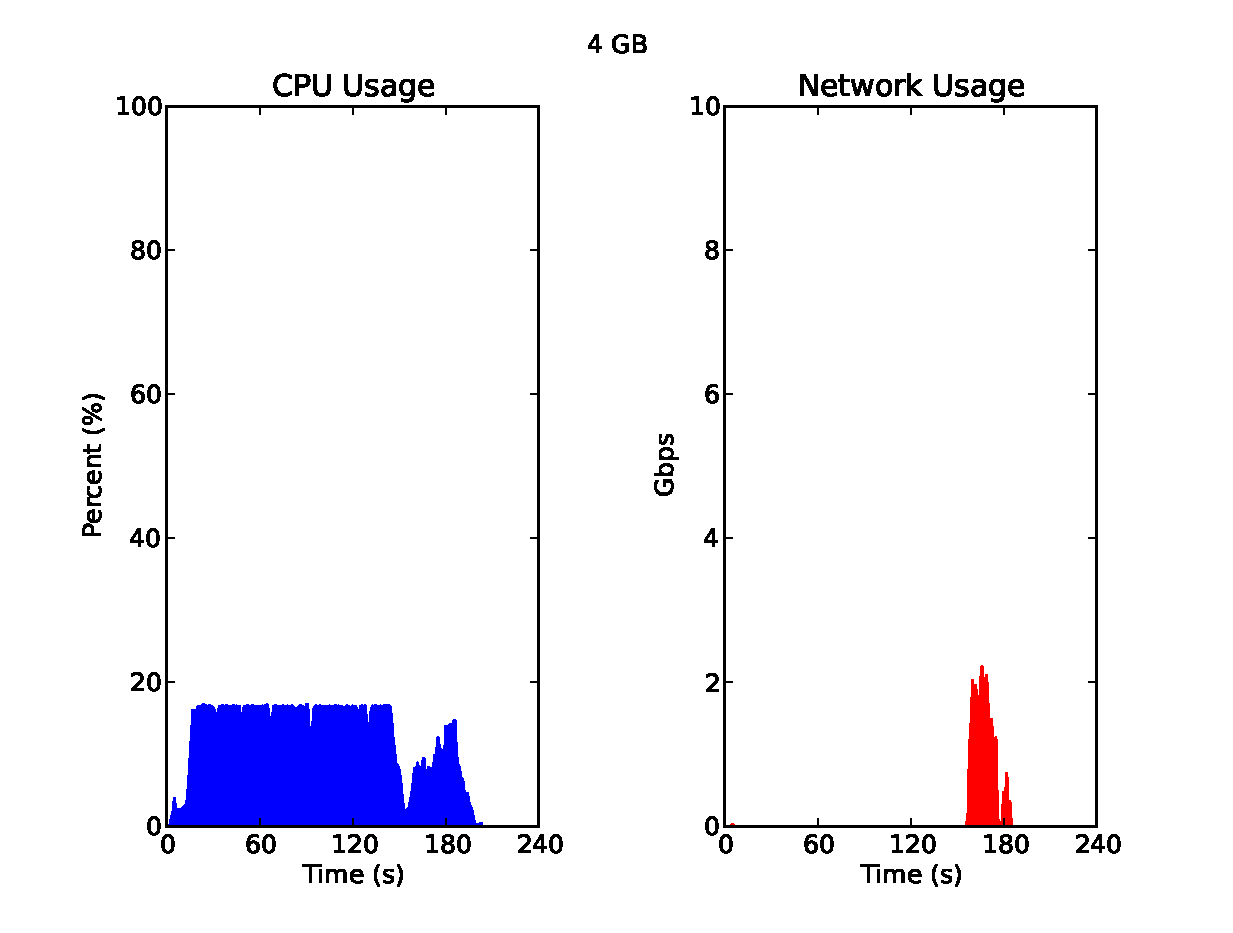
\includegraphics[width=\textwidth]{64maps_tcp.csv.eps}
                \caption{TCP}
                \label{fig:4GBsortrestcp}
        \end{subfigure}%
        \begin{subfigure}[b]{0.49\textwidth}
                \centering
                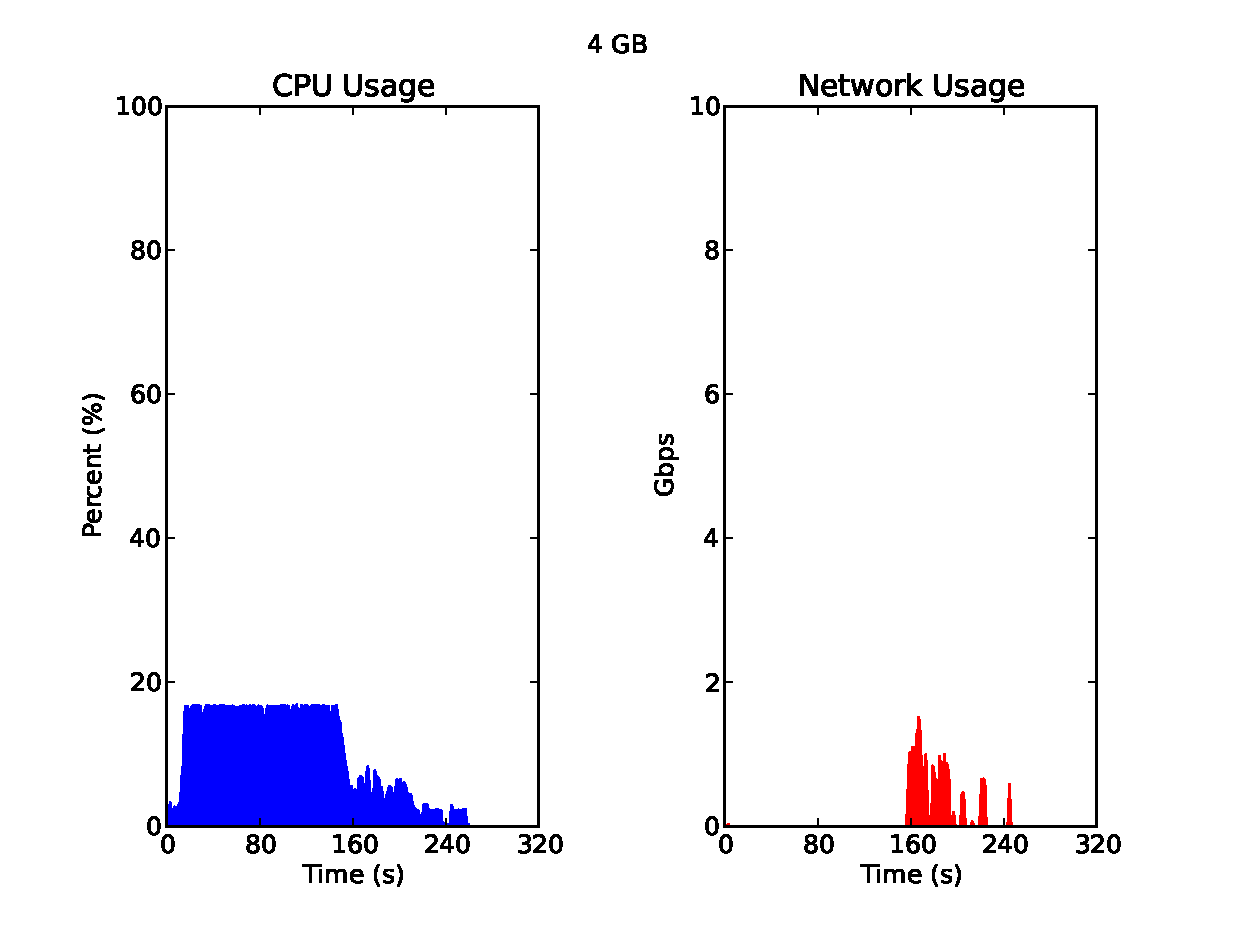
\includegraphics[width=\textwidth]{64maps_mptcp.csv.eps}
                \caption{MPTCP}
                \label{fig:4GBsortresmptcp}
        \end{subfigure}
        \caption{CPU and Network usage of sort using MPTCP for a 4 GB dataset}
        \label{chap:eval:sec:ciel:fig:sortresmptcp}
\end{figure}


\subsection{Delay-based vs. AQM-based congestion control}
\begin{figure}[h!]
  \centering
    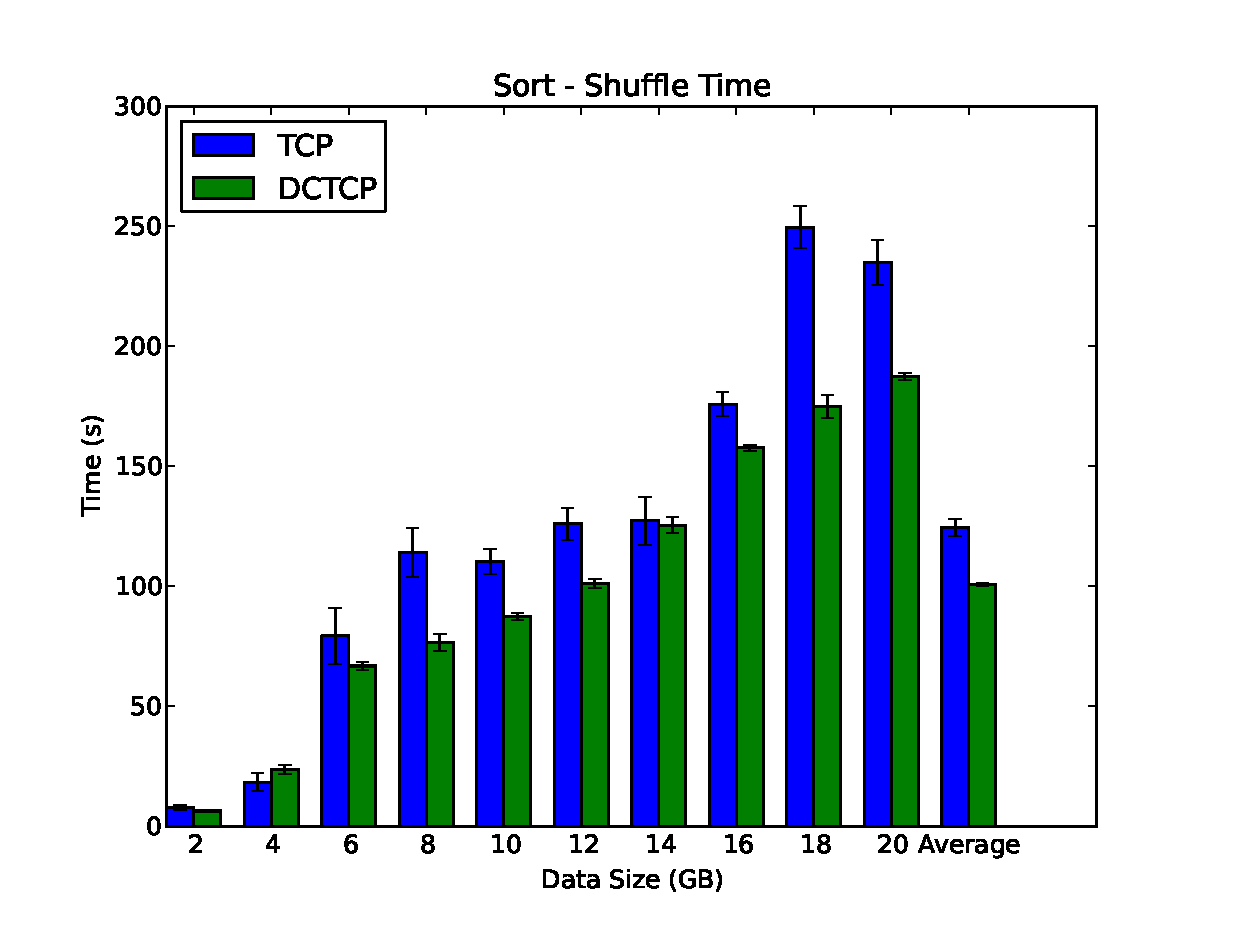
\includegraphics[width=0.8\textwidth]{shuffle_sort_dctcp.eps}
    \caption{Sort TCP vs. DCTCP - Shuffle Time - Star topology}
    \label{chap:eval:sec:ciel:fig:sortshuffledctcp}
\end{figure}

We now investigate whether active queue management (AQM)-based congestion
control can outperform the standard delay-based one. In the former, RTT
measurements are used as an indication of congestion while in the latter,
explicit feedback from the switches is employed. We use data center TCP
(DCTCP)\footnote{\url{https://github.com/myasuda/DCTCP-Linux}}~\cite{Alizadeh:2010:DCT}
as a representative protocol for AQM.
Figure~\ref{chap:eval:sec:ciel:fig:sortshuffledctcp} plots the performance of
standard delay-based TCP against AQM-based DCTCP on our sort application. DCTCP
reduces the shuffle time by 20\% on average as it achieves higher throughput.

Figure~\ref{chap:eval:sec:ciel:fig:sortresdctcp} shows the CPU and network
utilization under DCTCP. In contrast to
Figure~\ref{chap:eval:sec:ciel:fig:sortres} we see that network traffic spikes
are closely packed which results in higher throughput. This can be attributed to
DCTCP's ability to trade convergence for higher throughput. To achieve this,
DCTCP sources incrementally adjust their window size based on the extent of
congestion. In contrast, TCP throughput has more variation. At the same time we
note that TCP ensures more fairness for individual flows.
Table~\ref{chap:eval:sec:ciel:tab:jain} shows the Jain's fairness
index~\cite{Jain:1984:AQM} for both TCP and DCTCP. TCP's fairness is on average
0.05 higher than DCTCP. For shorter flows DCTCP does not converge quickly, as a
result it does not achieve fair share equilibrium. For larger flows the fairness
index of DCTCP matches that of TCP due to adequate time to converge to
equilibrium.

\begin{figure}[h!]
        \begin{subfigure}[b]{0.33\textwidth}
                \centering
                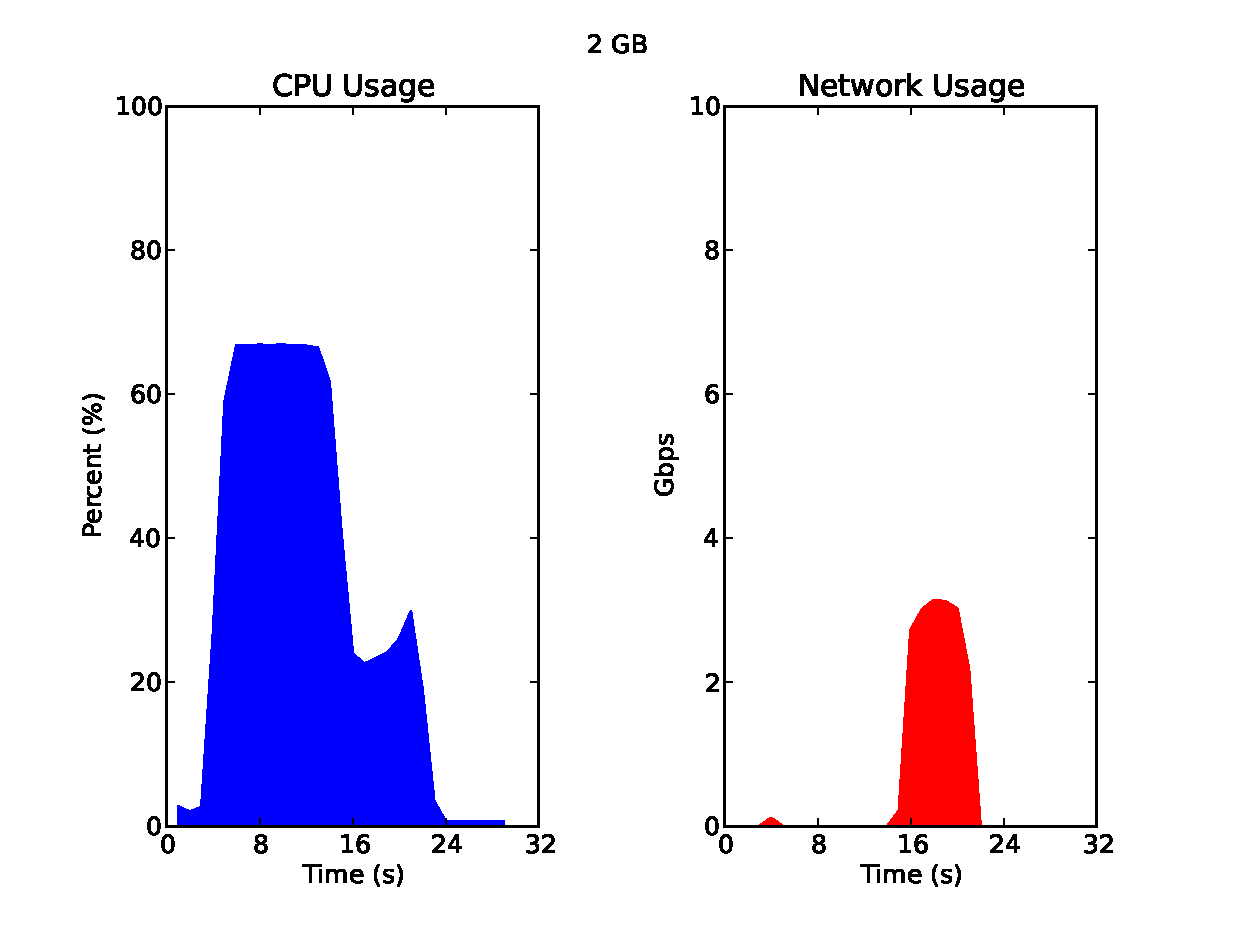
\includegraphics[width=\textwidth]{32maps_dctcp.csv.eps}
                \caption{2 GB - 32 maps}
                \label{fig:2GBsortresdctcp}
        \end{subfigure}%
        \begin{subfigure}[b]{0.33\textwidth}
                \centering
                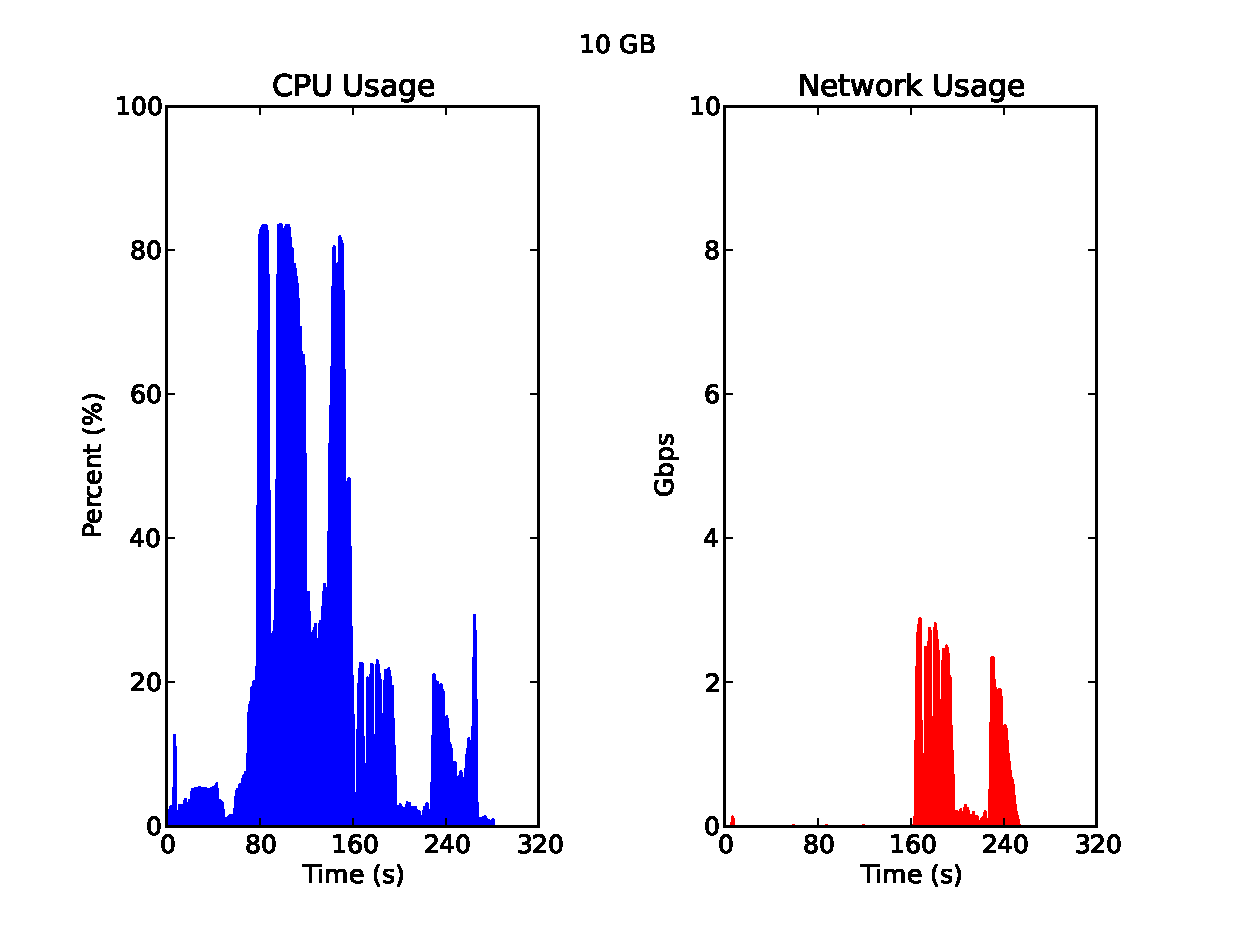
\includegraphics[width=\textwidth]{160maps_dctcp.csv.eps}
                \caption{10 GB - 160 maps}
                \label{fig:10GBsortresdctcp}
        \end{subfigure}
        \begin{subfigure}[b]{0.33\textwidth}
                \centering
                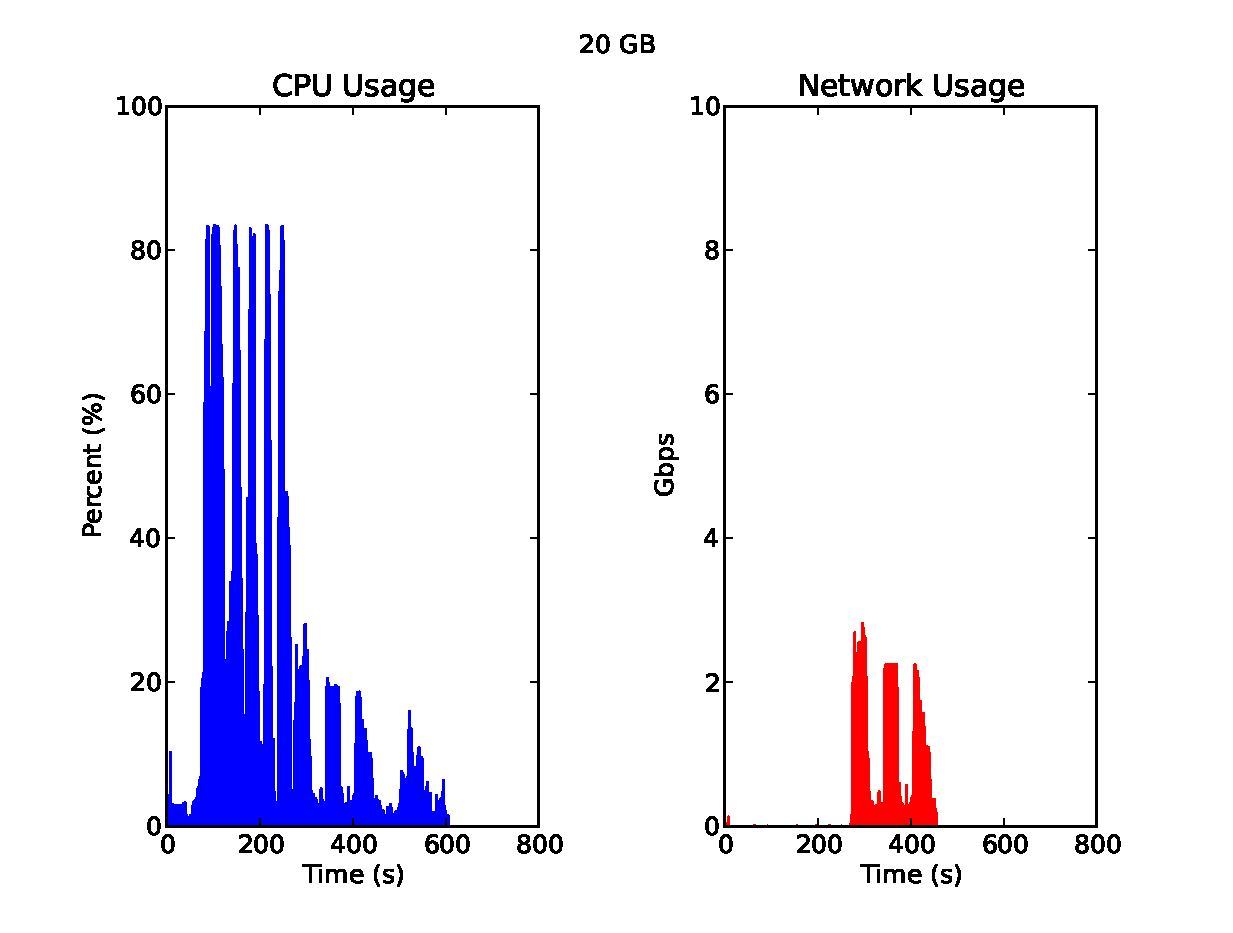
\includegraphics[width=\textwidth]{320maps_dctcp.csv.eps}
                \caption{20 GB - 320 maps}
                \label{fig:20GBsortresdctcp}
        \end{subfigure}
        \caption{CPU and Network usage of sort using DCTCP}
        \label{chap:eval:sec:ciel:fig:sortresdctcp}
\end{figure}

\begin{table}
                \centering
  \begin{tabular}{| l || l | l |}
    \hline
	\textbf{Data Size (GB)} & \textbf{DCTCP} & \textbf{TCP} \\ \hline
    2 & 0.799 & 0.793 \\ \hline
    4 & 0.902 & 0.904 \\ \hline
    6 & 0.801 & 0.943 \\ \hline
    8 & 0.759 & 0.964 \\ \hline
    10 & 0.896 & 0.938 \\ \hline
    12 & 0.910 & 0.945 \\ \hline
    14 & 0.924 & 0.968 \\ \hline
    16 & 0.940 & 0.965 \\ \hline
    18 & 0.958 & 0.969 \\ \hline
    20 & 0.944 & 0.955 \\ \hline \hline
    Average & 0.883 & 0.934 \\
    \hline
  \end{tabular}
  \caption{Jain's fairness index for DCTCP and TCP}
  \label{chap:eval:sec:ciel:tab:jain}
\end{table}

\subsection{Transport Encryption}
\begin{figure}[h!]
  \centering
    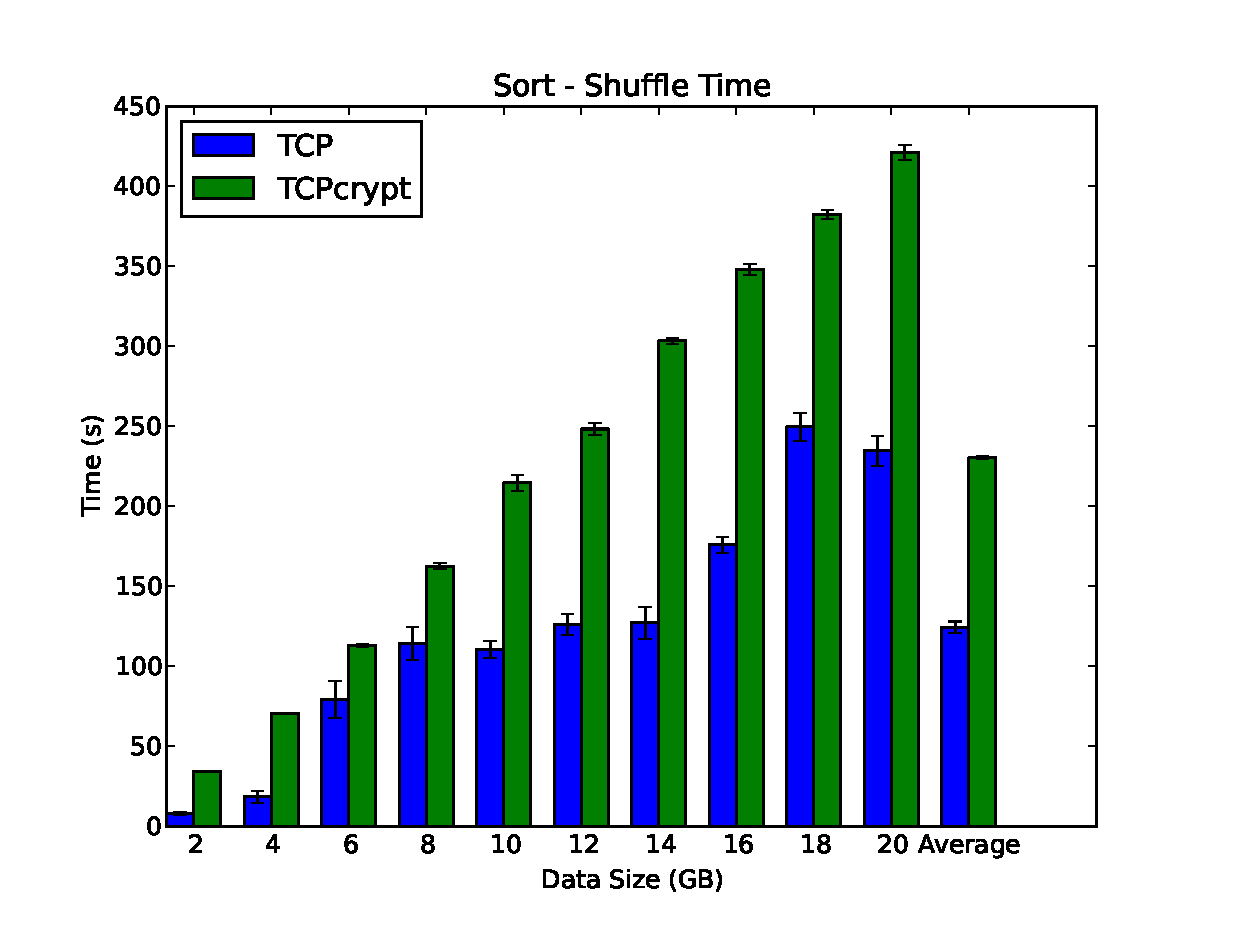
\includegraphics[width=0.8\textwidth]{shuffle_sort_tcpcrypt.eps}
    \caption{Sort TCP vs. TCPcrypt - Shuffle Time - Star topology}
    \label{chap:eval:sec:ciel:fig:sortshuffletcpcrypt}
\end{figure}
In cases where the same framework is being used by multiple users without any
VLAN isolation, users might want to protect their data by enforcing encryption.
This can be done at the application layer but that would result in a very high
overhead. We investigate whether transport layer encryption can be applied with
an acceptable overhead. We use
TCPcrypt\footnote{\url{https://github.com/sorbo/tcpcrypt}} as a representative
protocol and benchmark it against standard TCP.
Figure~\ref{chap:eval:sec:ciel:fig:sortshuffletcpcrypt} shows the shuffle time
of both protocols. On average, TCPcrypt results in an 85\% increase in data
transfer time. It is worth noting that we used the user-space implementation of
TCPcrypt. A kernel-space implementation would potentially decrease the overhead.

\begin{table}
  \centering
  \begin{tabular}{| l || l | l | l |}
    \hline
	\textbf{Receivers} & \textbf{Input size (GB)} & \textbf{Maps} &
	\textbf{Reduces}
	\\
	\hline
	10 & 2.5 & 40 & 10 \\ \hline
    20 & 5 & 80 & 20 \\ \hline
    30 & 7.5 & 120 & 30 \\ \hline
    40 & 10 & 160 & 40\\ \hline
    \hline
  \end{tabular}
  \caption{Parameters for concurrent flows experiment}
  \label{chap:eval:sec:ciel:tab:flows}
\end{table}

\begin{figure}[h!]
  \centering
    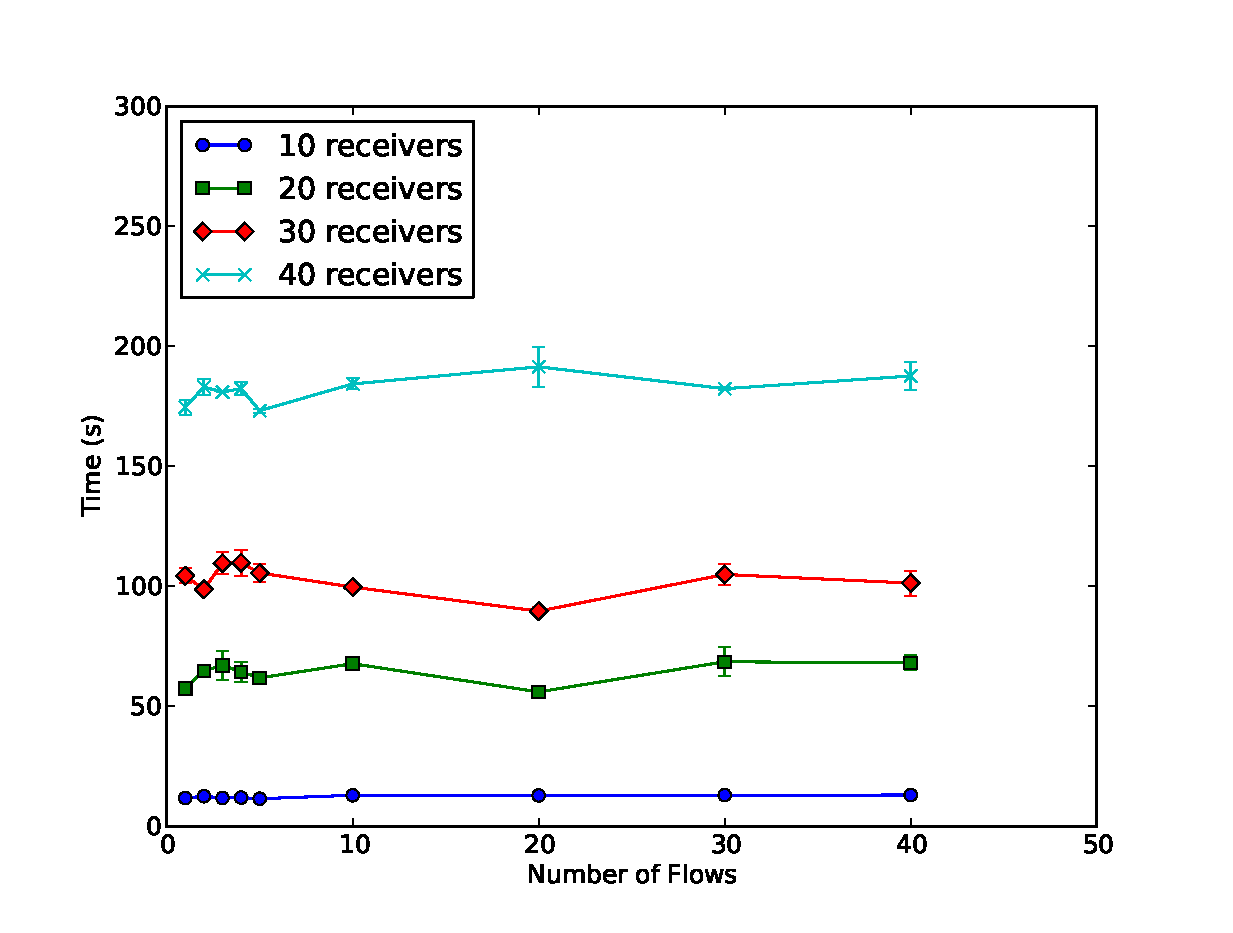
\includegraphics[width=0.8\textwidth]{shuffle_flows.eps}
    \caption{Shuffle time with increasing number of concurrent flows}
    \label{chap:eval:sec:ciel:fig:shuffleflows}
\end{figure}

\begin{figure}[h!]
  \centering
    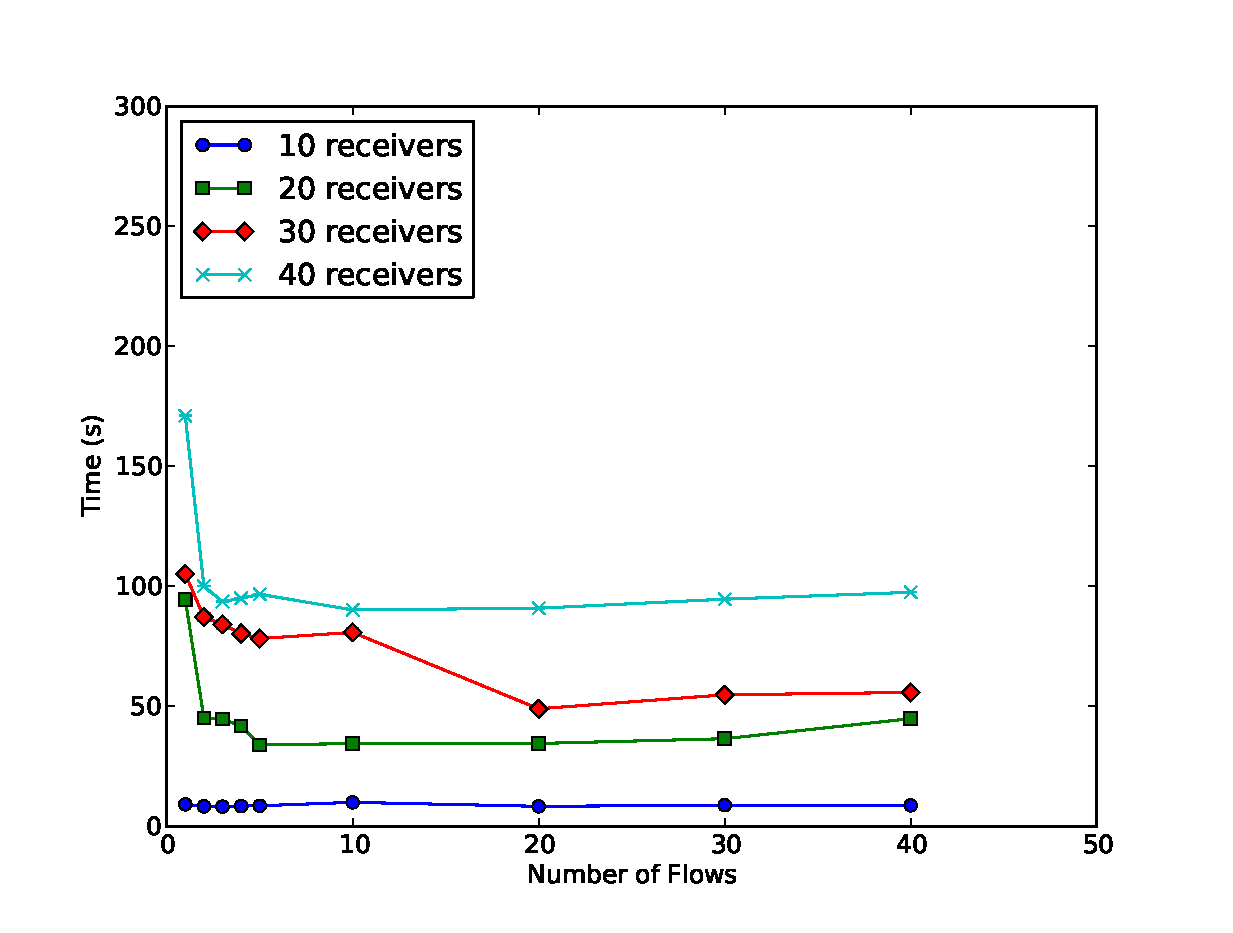
\includegraphics[width=0.8\textwidth]{shuffle_flows_jumbo.eps}
    \caption{Shuffle time with increasing number of concurrent flows using
    jumbo Ethernet frames}
    \label{chap:eval:sec:ciel:fig:shuffleflowsjumbo}
\end{figure}

\subsection{Number of concurrent flows}
In this experiment, we check the effect of varying the number of concurrent
connections at each worker to fetch its input during the shuffle phase. In
addition, we also study whether the number of receivers has any bearing on the
shuffle time. We vary the number of map and reduce tasks and the input data size
for our sort application (given in Table~\ref{chap:eval:sec:ciel:tab:flows}) to
force each reduce task to fetch approximately 256 MB of data.
Figure~\ref{chap:eval:sec:ciel:fig:shuffleflows} shows shuffle time for
increasing number of receivers as a function of the number of flows.
Surprisingly, the number of concurrent flows has no effect on the shuffle time.
To find out whether this is due to the nature of the application or our
experimental setup, we use
\texttt{iperf}\footnote{\url{http://sourceforge.net/projects/iperf/}} to measure
the throughput of concurrent senders. For even a small number of senders as 16,
the average throughput is 140.937 Mbps, which is far below the theoretical value
of 1 Gbps. Increasing the maximum transmission unit (MTU)\footnote{MTU is
maximum unit of data in bytes that is passed by any layer of the network stack.}
of Ethernet to 9000 byte jumbo frames~\cite{Chase:2000:ESO} substantially
increases the per sender/receiver pair throughput to 881.5 Mbps. Having achieved
full-bisection bandwidth between sender/receiver pairs, we repeat the original
experiment on our improved setup and plot the result in
Figure~\ref{chap:eval:sec:ciel:fig:shuffleflowsjumbo}. The results point to 3
main takeaways, (1) The effect of concurrent flows comes into play when the
receivers have to fetch more than one file from each sender, (2) Even having two
concurrent connections substantially improves performance, (3) Beyond a certain
point we encounter diminishing returns. In fact, due to the last point, systems
such as Hadoop limit the number of concurrent flows per receiver to
5\footnote{This limit is also set to keep the number of threads in check and
also to mitigate incast~\cite{Chowdhury:2011:MDT}.}. This analysis proves that
using the number of flows to implement weighted transport scheduling can effect
the shuffle time.
\begin{figure}[h!]
  \centering
    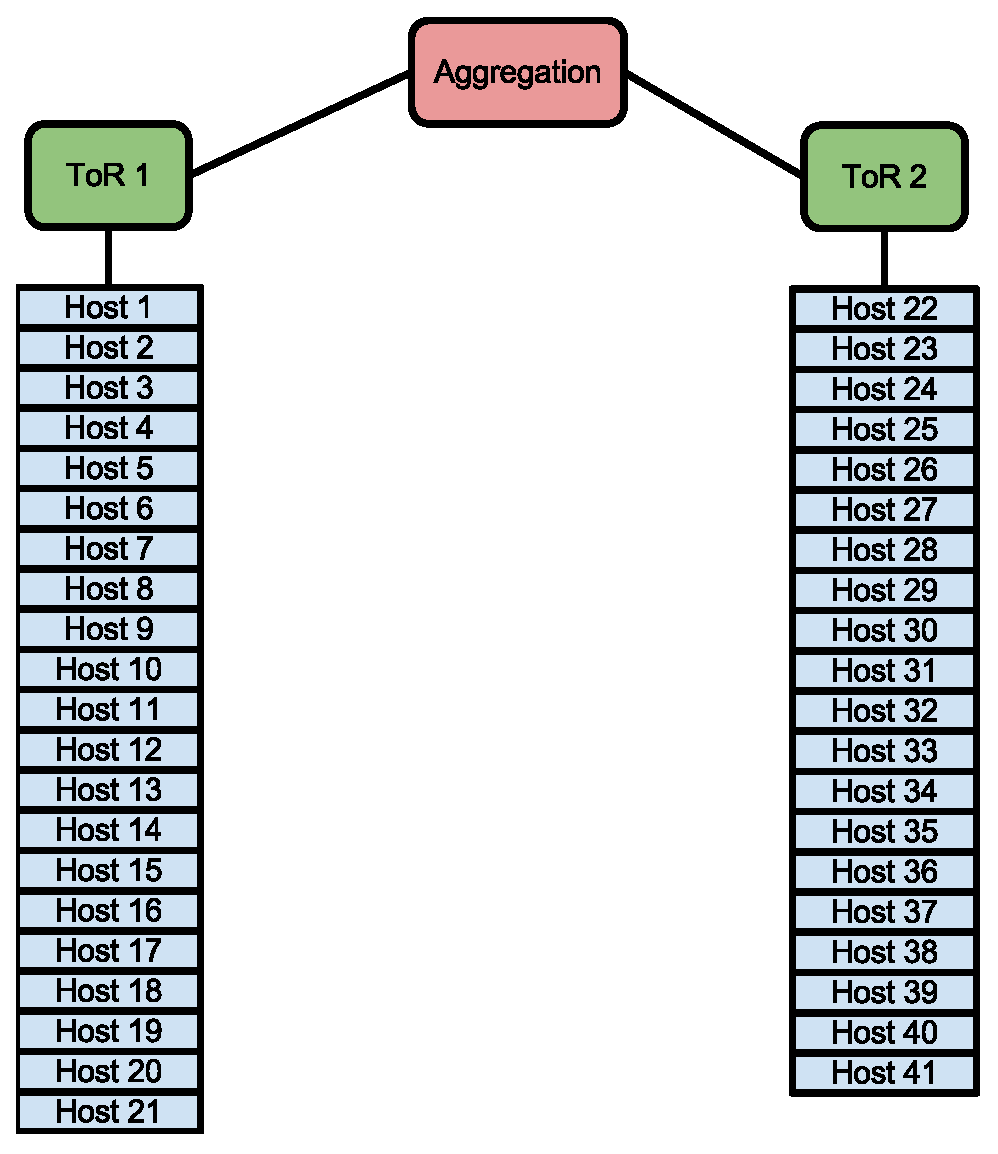
\includegraphics[width=0.3\textwidth]{2_rack_topology.eps}
    \caption{2 rack topology}
    \label{chap:eval:sec:ciel:fig:topology}
\end{figure}

\section{Performance of CIEL under Mission Control}
In this section, we evaluate the performance of CIEL under Mission Control for a
2 rack topology and 3 switches. Rack 1 has 21 hosts (containers) while Rack 2
has 20 hosts (containers). Hosts within each rack are connected via a 1 Gbps
switch each while the racks are connected via another 1 Gbps switch. The
topology is shown in Figure~\ref{chap:eval:sec:ciel:fig:topology}. The master is
run on a host in Rack 1 while the rest of the hosts in the two racks run
workers. We evaluate the performance of our sort application for different input
sizes. We first do the evaluation using the default TCP Flight Controller. We
then repeat the experiment by turning on ECN in all switches. This prompts
Mission Controller to switch to the DCTCP Flight Controller.
Figure~\ref{chap:eval:sec:ciel:fig:shuffle2racks} plots the shuffle time for
this experiment. On average, DCTCP results in a 9\% improvement in shuffle time.
DCTCP aims to keep switch buffer occupancies low by reacting to the extent of
congestion. By default, for a 1 Gbps network the queue length is limited to 20
packets or 30 KB. To corroborate this, we log the TCP receive queue length of
every worker every 125 ms for both TCP and DCTCP for an input data set of size
10 GB. Figure~\ref{chap:eval:sec:ciel:fig:queue} plots the time series of queue
length for a single worker. We see that DCTCP is able to keep the queue length
within 30 KB while the TCP receive queue is longer and has more variation. As a
result, DCTCP mitigates buffer pressure and does not allow a single flow to
overrun the shared buffer in the switch.


\begin{figure}[h!]
  \centering
    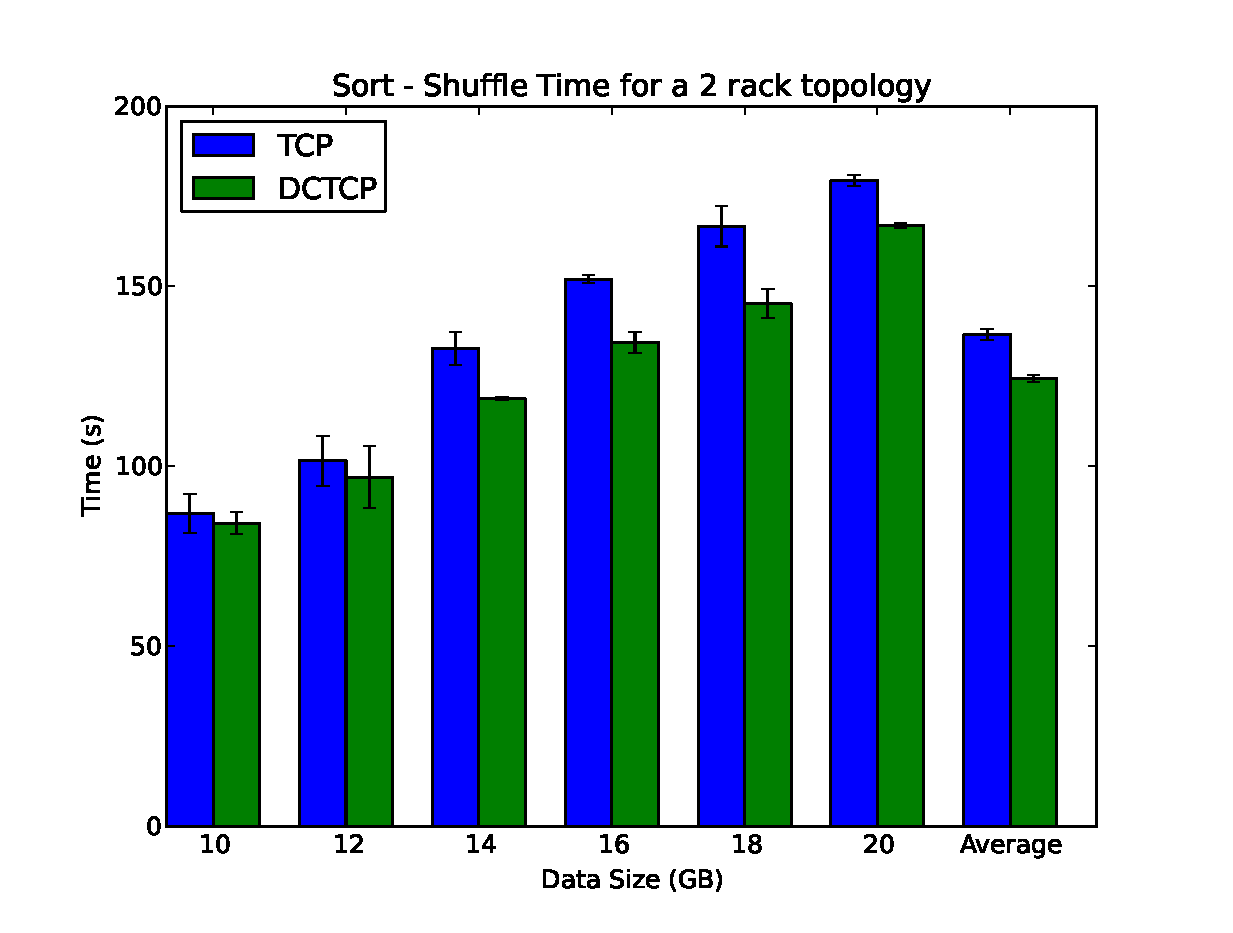
\includegraphics[width=0.8\textwidth]{shuffle_sort_dctcp_2racks.eps}
    \caption{Shuffle time for TCP and DCTCP on a two rack topology}
    \label{chap:eval:sec:ciel:fig:shuffle2racks}
\end{figure}

\begin{figure}[h!]
        \begin{subfigure}[b]{0.49\textwidth}
                \centering
                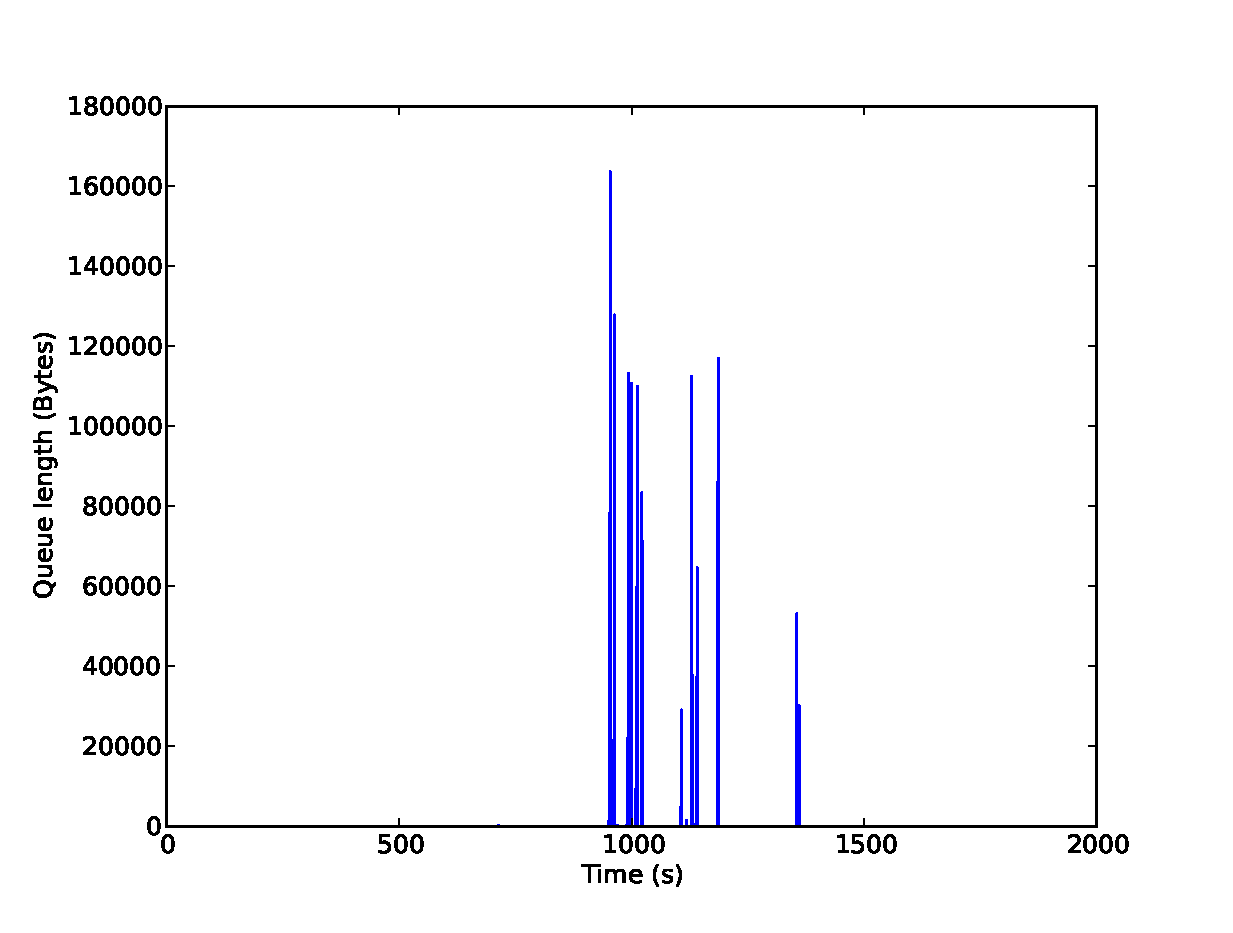
\includegraphics[width=\textwidth]{q_tcp.eps}
                \caption{TCP}
                \label{fig:tcpq}
        \end{subfigure}%
        \begin{subfigure}[b]{0.49\textwidth}
                \centering
                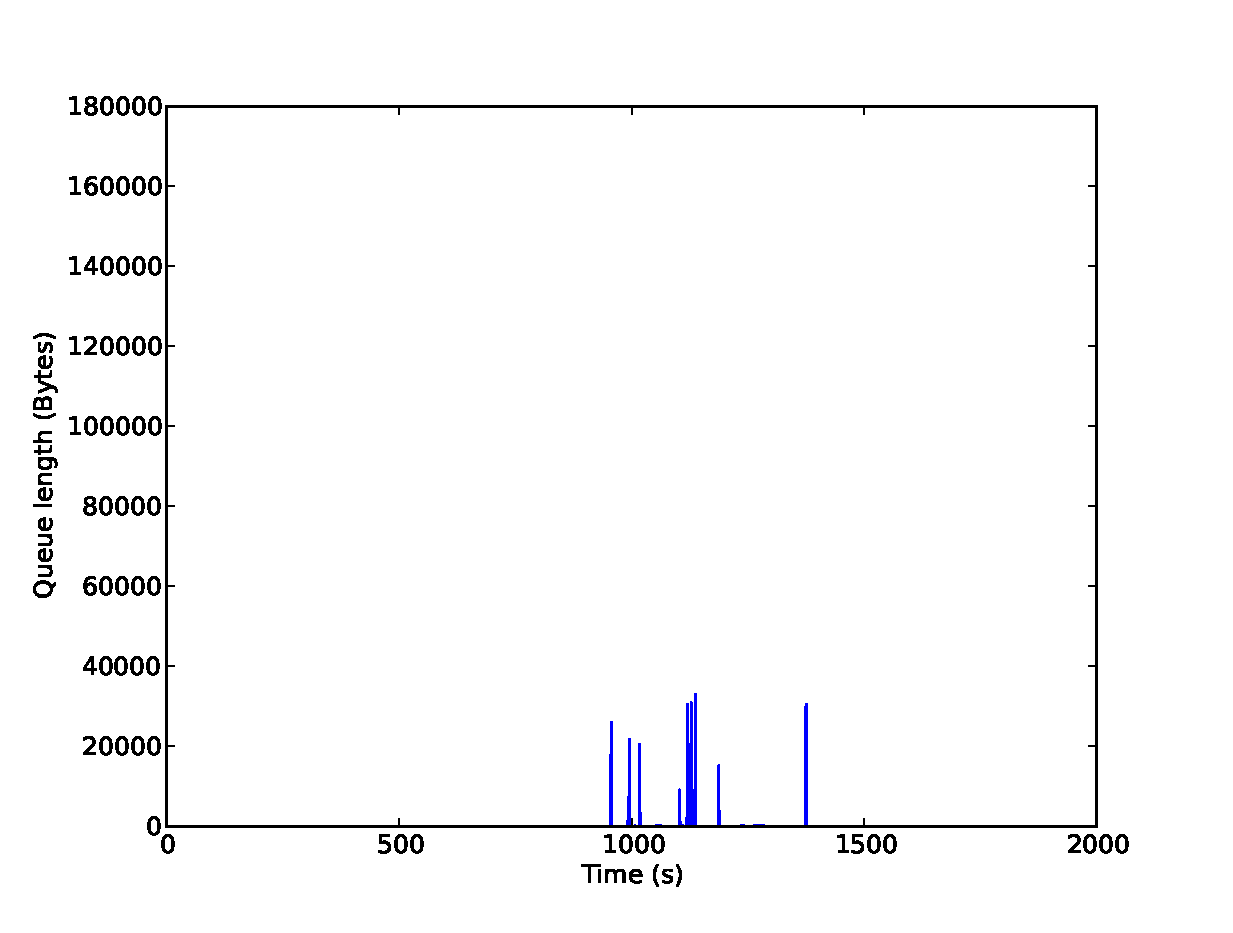
\includegraphics[width=\textwidth]{q_dctcp.eps}
                \caption{DCTCP}
                \label{fig:dctcpq}
        \end{subfigure}
        \caption{Time series of receive queue length for TCP and DCTCP}
        \label{chap:eval:sec:ciel:fig:queue}
\end{figure}

\section{Summary}
Overall, the evaluation shows that concurrent flow assignment is a practical
method of allocating network resources. In addition, transport protocol
performance and usefulness can vary depending on application semantics and user
requirements. Finally, it is possible for a data intensive computing framework
to delegate its data transfer to an abstraction layer without requiring any
architectural changes to the framework itself or the applications which execute
atop it.

\chapter{Summary and Conclusions}\label{chapter:conclusion}
It is a well-known fact that TCP is sub-optimal inside the data center as it was
originally designed for a wide-area network with radically different
requirements and settings. A number of different solutions have been recently
proposed with the aim to address the shortcomings of TCP in the data center.
These vary from novel topologies to protocols which take advantage of multiple
paths in the network. Unfortunately, there is no one-size-fits-all solution. To
remedy this, in this thesis we presented, Mission Control, an abstraction layer
that maintains global state to choose the semantics of data transfers in data
intensive computing frameworks. To this end, it uses application semantics, user
constraints, runtime parameters, and network characteristics to select an
appropriate transport protocol and data transfer schedule. It is capable of
using different policies to allocate network resources to different transfers.
In addition, it supports a range of transport protocols to enable diversity. The
evaluation presented in this thesis corroborates our position that there is no
transport regime which is optimal across the board. In summary, the main
contributions of this thesis are the following:

\begin{enumerate}
  \item Analysis of common communication patterns in the data center and
  relevant literature to prove that TCP is sub-optimal in the data center
  \item Design and implementation of Mission Control, which enables
  data intensive computing frameworks to delegate data transfer mechanism and
  policy
  \item Evaluation of CIEL under different transport semantics and insight into
  data transfer operation
\end{enumerate}

The biggest contribution of Mission Control is the framework itself which allows
any transport protocol, current or future, to be used by batch-processing
systems without requiring any changes to the systems or the applications.
Thus, Mission Control is a means to an end: Decoupling data transfer mechanism
from policy in the data center. We conclude by listing possible future work:

\begin{itemize}
  \item Recent work~\cite{Smith:2012:TCF} has shown that I/O throughput
	and latency can vary significantly (order of magnitude) due to the underlying
	IPC mechanism, the physical and virtual architecture, and OS primitives.
	Mission Control can be run on top of the proposed \textsc{fable} stack to
	switch to shared memory primitives if the destination is local.
   \item Mission Control can be merged with Quincy~\cite{Isard:2009:QFS} and
   Mesos~\cite{Hindman:2011:MPF} to enable data center/cluster-wide CPU, memory
   and I/O isolation and scheduling.
   \item It would interesting to see how Mission Control can be used to leverage
   the transparency of the software stack in Akaros~\cite{Rhoden:2011:IPE} to
   improve I/O performance.
   \item 80\% of the traffic in a cluster stays within a
   rack~\cite{Benson:2010:NTC}. This information can be used by Mission Control
   to assign more flows to in-rack transfers.
   \item In this thesis we only considered an environment under the operational
	control of a single domain. It is not clear how different transport protocols
	would interact with each other within the same data center. For instance,
	DCTCP flows might not ensure fairness to TCP flows~\cite{Alizadeh:2010:DCT}.
	\item Our focus in this discussion was on batch-processing systems which
	require high throughput. In addition to the systems, data centers also run
	stream processing systems, such as S4~\cite{Neumeyer:2010:SDS} and
	Percolator~\cite{Peng:2010:LIP}, which require low latency. The choice of
	underlying transport semantics for these systems is completely different and
	Mission Control would need to be made aware of these requirements.
	\item The last point can be generalized to a trade-off between bandwidth and
	latency. Protocols such as HULL~\cite{Alizadeh:2012:LIM} make this trade-off
	possible. Mission Control can be extended to use global knowledge to optimize
	this trade-off.
	\item Mission Control currently supports 4 different transport protocols but
	the framework is flexible enough to be extended to make use of more protocols
	such as Deadline-Driven Delivery (D$^3$)~\cite{Wilson:2011:BNL}, Structured Stream
	Transport (SST)~\cite{Ford:2007:SSN}, and ICTCP~\cite{Wu:2010:IIC}.
\end{itemize}

\appendix
\singlespacing

\bibliographystyle{unsrt} 
\bibliography{dissertation} 

\end{document}
